\documentclass[12pt, a4paper]{report}
\usepackage{graphicx, array, amsthm, amssymb, amsmath, algorithm, algpseudocode, float, xcolor, thmtools, thmbox}
\usepackage[english]{babel}

\makeatletter
\renewcommand\thmbox@headstyle[2]{\bfseries #1}
\makeatother
\newtheorem[style=M,bodystyle=\normalfont]{proposition}{Proposition}
\newtheorem[style=M,bodystyle=\normalfont]{theorem}{Theorem}
\newtheorem[style=M,bodystyle=\normalfont]{corollary}{Corollary}
\newtheorem[style=M,bodystyle=\normalfont]{lemma}{Lemma}
\newtheorem[style=M,bodystyle=\normalfont]{definition}{Definition}


\title{Foundation Of Operations Research \\ \textit{Theory}}
\author{Christian Rossi}
\date{Academic Year 2023-2024}

\begin{document}

\maketitle

\newpage

\begin{abstract}
    Operations Research is the branch of applied mathematics dealing with quantitative methods to analyze and solve
    complex real-world decision-making problems. 
    
    The course covers some fundamental concepts and methods of Operations Research pertaining to graph optimization, 
    linear programming and integer linear programming. 
    
    The emphasis is on optimization models and efficient algorithms with a wide range of important applications in 
    engineering and management.  
\end{abstract}

\newpage

\tableofcontents

\newpage
 
\chapter{Introduction}
    \section{Definition}
    \begin{definition}
        \emph{Operations Research} is the branch of mathematics in which mathematical models and quantitative methods are used to analyze complex decision-making problems and find
        near-optimal solutions.
    \end{definition}
    It is an interdisciplinary field at the interface of applied mathematics, computer science, economics and industrial engineering. 

    \section{Decision-making problems}
    \begin{definition}
        The \emph{decision-making problems} are problems in which we must choose a feasible solution among many alternatives based on one or several criteria. 
    \end{definition}
    The more complex decision-making problems are tackled via a mathematical modelling approach. 
    Those problems can be classified in the following categories: 
    \begin{enumerate}
        \item Assignment problem: given $m$ jobs and $m$ machines, suppose that each job can be executed by any machine and that $t_{ij}$ is the execution time of job $J_i$ one
            machine $M_j$. We want to decide which job assign to each machine to minimize the total execution time. Each job must be assigned to exactly one machine, and each 
            machine to exactly one job. The number of feasible solution is equal to $m!$. 
        \item Network design: we want to decide how to connect $n$ cities via a collection of possible links to minimize the total link cost. 
            Given a graph $G=(N,E)$ with a node $i \in N$ for each city and an edge $\{i,j\} \in E$ of cost $c_ij$, select a subset of edges of minimum total cost, guaranteeing that 
            all pairs of nodes are connected. The number of feasible solution is equal to $2^{\left\lvert E \right\rvert}$. 
        \item Shortest path: given a direct graph that represents a road network with distances (traveling times) for each arc, determine the shortest path between two points (nodes).
        \item Personnel scheduling: determine the week schedule for the hospital personnel, to minimize the number of people involved while meeting the daily requirements.
        \item Service management: determine how many desks to open at a given time of the day so that the average customer waiting time does not exceed a certain value. 
        \item Multi-criteria problem: decide which laptop to buy considering the price, the weight and the performance. 
        \item Maximum clique (community detection in social networks): determine the complete sub-graph of a graph, with the maximum number of vertices.
    \end{enumerate}

    \section{History}
    In the World War II, teams of scientists were asked to do research on the most efficient way to conduct the operations.
    In the decades after the war, the techniques became public and began to be applied more widely to problems in business, industry and society.
    During the industrial boom, the substantial increase in the size of the companies and organizations gave rise to more complex decision-making problems thanks to
    fast progress in Operations Research and in numerical analysis methodologies and advent and diffusion of computers. 

    \section{Operations Research workflow}
    \begin{figure}[H]
        \centering
        
\includegraphics[width=1\linewidth]{images/study.png}
    \end{figure}
    The main steps in studying an Operations Research problem are: 
    \begin{enumerate}
        \item Define the problem.
        \item Build the model.
        \item Select or develop an appropriate algorithm. 
        \item Implement it or use an existing program. 
    \end{enumerate}
    After all this process we need to analyze the results with feedbacks. 

    The model obtained with this process is a simplified representation of a real-world problem. To define it we must identify the fundamental elements of the problem and the main
    relationships among them. 
    \begin{example}
        A company produces three types of electronic devices: $D_1,D_2,D_3$, going through three main phases of the production process: assembly, refinement and quality control.
        The time required for each phase and product is: 
        \begin{table}[H]
            \centering
            \begin{tabular}{c|ccc|}
            \cline{2-4}
            \textbf{}                             & \textbf{$D_1$} & \textbf{$D_2$} & $D_3$ \\ \hline
            \multicolumn{1}{|c|}{Assembly}        & 80             & 70             & 120   \\
            \multicolumn{1}{|c|}{Refinement}      & 70             & 90             & 20    \\
            \multicolumn{1}{|c|}{Quality control} & 40             & 30             & 20    \\ \hline
            \end{tabular}
        \end{table}
        The available resources within the planning horizon in minutes are: 
        \begin{table}[H]
            \centering
            \begin{tabular}{|c|c|c|}
            \hline
            \textbf{Assembly} & \textbf{Refinement} & \textbf{Quality control} \\ \hline
            30 000            & 25 000              & 18 000                   \\ \hline
            \end{tabular}
        \end{table}
        The unary product for each product in: 
        \begin{table}[H]
            \centering
            \begin{tabular}{|c|c|c|}
            \hline
            $D_1$          & $D_2$          & $D_3$ \\ \hline
            1600           & 1000           & 2000  \\ \hline
            \end{tabular}
        \end{table}
        The main assumption is that the company can sell whatever it produces. 

        The mathematical model that describes the problem given before is the following: 
        \begin{itemize}
            \item Decision variables: $x_j$ is the number of devices $D_j$ produced for $j=1,2,3$.
            \item Objective function: we need to maximize the earning, so we have: 
                \[\max{\left[1.6x_1+1x_2+2x_3\right]}\]
            \item Constraints: they are on the production limit of each phase, that are: 
                \[80x_1+70x_2+120x_3 \leq 30000\]
                \[70x_1+90x_2+20x_3 \leq 25000\]
                \[40x_1+30x_2+20x_3 \leq 18000\]
            \item Variable type: the variables must be non-negative values, so we have $x_1,x_2,x_3 \geq 0$.
        \end{itemize}
    \end{example}
    \begin{example}
        An insurance company must decide which investments to select out of a given set of possible assets.
        \begin{table}[H]
            \centering
            \begin{tabular}{|c|ccc|}
            \hline
            \textbf{Investments} & \textbf{Area} & \textbf{Capital ($c_j$)} & \textbf{Return ($r_j$)} \\ \hline
            A (automotive)       & Germany       & $150 000$                & $11\%$                  \\
            B (automotive)       & Italy         & $150 000$                & $9\%$                   \\
            C (ICT)              & USA           & $60 000$                 & $13\%$                  \\
            D (ICT)              & Italy         & $100 000$                & $10\%$                  \\
            E (real estate)      & Italy         & $125 000$                & $8\%$                   \\
            F (real estate)      & France        & $100 000$                & $7\%$                   \\
            G (treasury bonds)   & Italy         & $50 000$                 & $3\%$                   \\
            H (treasury bonds)   & UK            & $80 000$                 & $5\%$                   \\ \hline
            \end{tabular}
        \end{table}
        The available capital is $600\:000$ euro. It is required to take at most five different investments. It is also required to take at maximum three investments in Italy and 
        maximum three abroad. 

        The mathematical model that describes the problem given before is the following:
        \begin{itemize}
            \item Decision variables: boolean value to communicate if the investment is selected or not: $x_j=1$ if the $j$-th investment is selected and $x_j=0$ otherwise, for
                $j=0,\dots, 8$.
            \item Objective function: we need to maximize the expected return, so we have: 
                \[\max{\left[\sum_{j=1}^8{c_jr_jx_j}\right]}\]
            \item Constraints: there is a constraint on the capital that insurance
                \[\sum_{j=1}^8{c_jx_j} \leq 800\]
                There is a constraint also on the max number of general investment and on the region they are coming from formalized asked
                \[\sum_{j=1}^8{x_j} \leq 5\]
                \[x_2+x_4+x_5+x_7 \leq 3\]
                \[x_1+x_3+x_6+x_8 \leq 3\]
            \item Variable type: the variables are binary integer defined as $x_j \in \{0,1\} \:\: 1 \leq j \leq 8$. 
        \end{itemize}
        The variant requires that if any of the ICT investment is selected, then at least one of the treasury bond must be select. This requires one new constraint that is: 
        \[\dfrac{x_3+x_4}{2} \leq x_7+x_8\]
        It is divided by two because if both ICT are selected at least one treasury bound must be selected and not two. 
    \end{example}
    \begin{example}
        Consider three oil pits, located in positions $A=(0,0)$, $B=(300,0)$, and $C=(240,300)$, from which oil is extracted. 
        \begin{figure}[H]
            \centering
            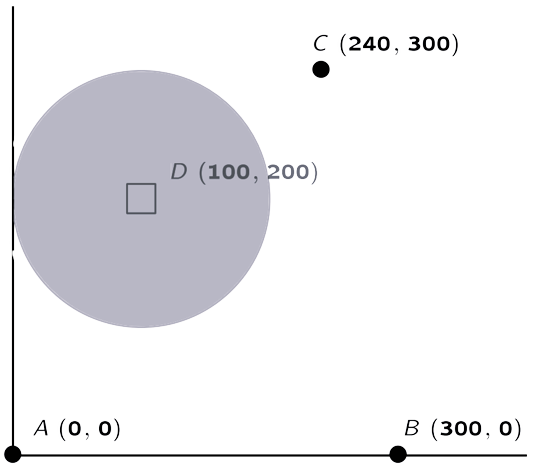
\includegraphics[width=0.4\linewidth]{images/example3.png}
        \end{figure}
        Connect them to a refinery with pipelines whose cost is proportional to the square of their length. The refinery must be at least 100 km away from point $D=(100,200)$, but 
        the oil pipelines can cross the corresponding forbidden zone. Give a mathematical model to decide where to locate the refinery to minimize the total pipeline cost. 
        \begin{itemize}
            \item Decision variables: the coordinates of the refinery $x_1,x_2$. 
            \item Objective function: we need to minimize the cost, so we have: 
            \begin{align*}
                \min{z} &=\left[ (x_1-0)^2+(x_2-0)^2 \right] \\
                        &+ \left[ (x_1-300)^2+(x_2-0)^2 \right] \\
                        &+ \left[ (x_1-240)^2+(x_2-300)^2 \right] 
            \end{align*}
            \item Constraints: there is a constraint on the location that is
                \[\sqrt{{\left( x_1-100 \right)}^2+{\left( x_2-100 \right)}^2} \geq 100\]
            \item Variable type: $x_1,x_2 \in \mathbb{R}$
        \end{itemize}
    \end{example}

    \section{Mathematical programming problem}
    \begin{table}[H]
        \centering
        \begin{tabular}{c|ccc|}
        \cline{2-4}
                                                                   & \textbf{Decisions} & \textbf{Objective} & \textbf{Uncertainty} \\ \hline
        \multicolumn{1}{|c|}{\textit{Mathematical programming}}    & single                   & one                          & -                    \\
        \multicolumn{1}{|c|}{\textit{Multi-objective programming}} & single                   & multiple                     & -                    \\
        \multicolumn{1}{|c|}{\textit{Stochastic programming}}      & -                        & -                            & $\checkmark$         \\
        \multicolumn{1}{|c|}{\textit{Game theory}}                 & multiple                 & -                            & -                    \\ \hline
        \end{tabular}
    \end{table}
    We will analyze the mathematical programming problems. 
    The optimization usually requires to minimizing or maximizing a given function. 
    Note that maximizing $f(x)$ is the same problem of minimizing $-f(x)$. The problems are characterized by: 
    \begin{itemize}
        \item Decision variables $x \in \mathbb{R}^n$: numerical variables that identify a solution. 
        \item Feasible region $X \subseteq \mathbb{R}^n$.
        \item Objective function $f:X \rightarrow\mathbb{R}$: expresses in quantitative terms the value of each feasible solution. 
    \end{itemize}
    Solving a mathematical programming problem consists in finding a feasible solution which is globally optimum. It may happen that: the problem is infeasible, unbounded, has a single 
    optimal solution or has numerous optimal solutions. 
    When the problem is very hard we must settle for a feasible solution that is a local optimum. An optimization problem can have many local optima. 
    Mathematical programming can be classified in:
    \begin{enumerate}
        \item Linear Programming.
        \item Integer Linear Programming.
        \item Nonlinear Programming. 
    \end{enumerate}
    
    Multi-objective programming can be taken into account in different ways. Suppose we wish to minimize $f_1(x)$ and maximize $f_2(x)$, we can: 
    \begin{enumerate}
        \item Turn it into a single objective problem by expressing the two objectives in terms of the same unit: 
            \[\min{\lambda_1f_1(x)-\lambda_2f_2(x)}\]
            for appropriate scalars $\lambda_1$ and $\lambda_2$.
        \item Optimize the primary objective function and turn the other objective into a constraint: 
            \[\max_{x \in X}f_2(x) \:\:\:\: f_1(x)\leq \epsilon\]
            for an appropriate constant $\epsilon$. 
    \end{enumerate}

\newpage

\chapter{Algorithms}
    \section{Complexity}
    \begin{definition}
        An \emph{algorithm} is a sequence of instructions that allows to solve any instance of a problem.
    \end{definition}
    The execution time of an algorithm depends on the instance and on the computer. We want to evaluate the complexity of the algorithm as a function of the size of the instance
    independently of the hardware. Thus, we consider the number of elementary operations and assume all have the same cost. Since it is usually hard to determine the exact number of
    elementary operations. We consider the asymptotic number of elementary operations in the worst case: we look for a function $f(n)$ which is asymptotically an upper bound on 
    number of elementary operations needed to solve any instance of size at most $n$. 
    \begin{definition}
        A function $f$ is \emph{ordered} of $g$, written $f(n)=O(g(n))$, if $\exists c > 0$ such that $f(n) \leq cg(n)$, for $n$ sufficiently large. 
    \end{definition}
    Two classes of algorithms are distinguished according to their worst-case complexity:
    \begin{itemize}
        \item Polynomial: $O(n^d)$ for a given constant $d$.
        \item Exponential: $O(2^n)$. 
    \end{itemize}
    Algorithms with a high order polynomial complexity are not efficient in practice.
    \begin{figure}[H]
        \centering
        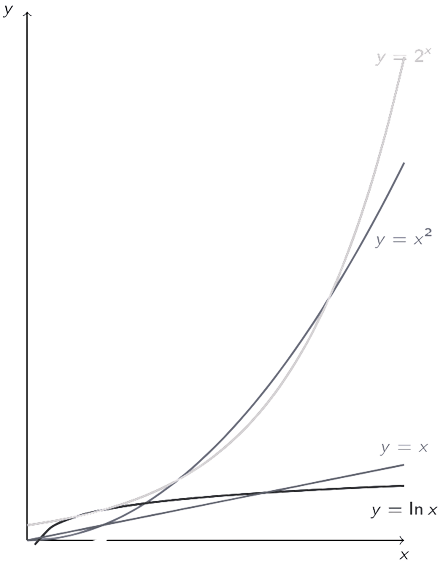
\includegraphics[width=0.25\linewidth]{images/complexity.png}
        \caption{Plot of various algorithm's complexity}
    \end{figure}
    \begin{definition}
        The \emph{size of an instance} $I$, $\left\lvert I \right\rvert$ is the number of bits needed to describe the instance. 
    \end{definition}

    \section{Definitions}
    \begin{definition}
        An algorithm is \emph{exact} if it provides an optimal solution for every instance. 
        
        An algorithm is \emph{heuristic} if it does not provide an optimal solution for every instance.

        A \emph{greedy algorithm} constructs a feasible solution iteratively by making at each step a locally optimal choice, without reconsidering previous choices. 
    \end{definition}

    \section{Dynamic programming}
    Dynamic programming was proposed by Richard Bellman in 1953 as a general technique in which an optimal solution, composed of a sequence of elementary decisions, is determined 
    by solving a set of recursive equations. So, dynamic programming is applicable to any sequential decision problem for which the optimality property is satisfied. 
    
    It is used nowadays in multiple sectors: optimal control, equipment maintenance and replacement, selection of inspection points along a production line. 

\newpage

\chapter{Network optimization models}
    \section{Introduction}
    Many decision-making problems can be formulated in terms of graphs.
    \begin{definition}
        A \emph{graph} is a pair $G=(N,E)$, with a set of nodes $N$ and a set of edges or arcs $E \subseteq N \times N$ connecting them pairwise. 

        An edge connecting the nodes $i$ and $j$ is represented by $\{i,j\}$ or $(i,j)$ if the graph is \emph{undirected} or \emph{directed} respectively. 
    \end{definition}
    \begin{example}
        A road network which connects $n$ cities can be modelled by a graph where a city corresponds to a node, and a connection corresponds to an edge. 
        \begin{figure}[H]
            \centering
            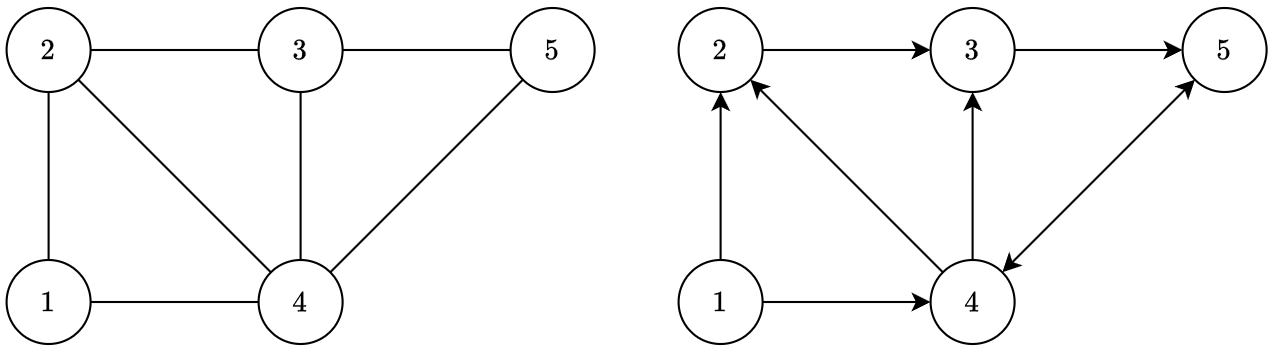
\includegraphics[width=0.75\linewidth]{images/graph.png}
        \end{figure}
        The graph on the left is undirected and defined as: 
        \begin{itemize}
            \item $N=\{1,2,3,4,5\}$
            \item $E=\{\{1,2\},\{1,4\},\{2,3\},\{2,4\},\{3,4\},\{3,5\},\{4,5\}\}$
        \end{itemize}
        The graph on the right is directed and defined as: 
        \begin{itemize}
            \item $N=\{1,2,3,4,5\}$
            \item $E^{'}=\{(1,2),(1,4),(2,3),(2,4),(3,4),(3,5),(4,5)\}$
        \end{itemize}
    \end{example}
    \begin{definition}
        Two nodes are \emph{adjacent} if they are connected by an edge. 
        
        An edge $e$ is \emph{incident} in a node $v$ if $v$ is an endpoint of $e$. 
        
        In undirected graphs, the \emph{degree} of a node is the number of incident edges in a given node. 
        
        In directed graph, the \emph{in-degree} (\emph{out-degree}) of a node is the number of arcs that ave it as successor (predecessor).
    \end{definition}
    \begin{example}

        In the undirected graph, we have that nodes $1$ and $2$ are adjacent and $1$ and $3$ are not. The edge $\{1,2\}$ is incident in nodes $1$ and $2$. Node $1$ has a degree $2$,
        and node $4$ has a degree of $4$. 

        In the directed graph, the node $1$ has an in-degree equal to $0$, and an out-degree equal to $2$.
        \begin{figure}[H]
            \centering
            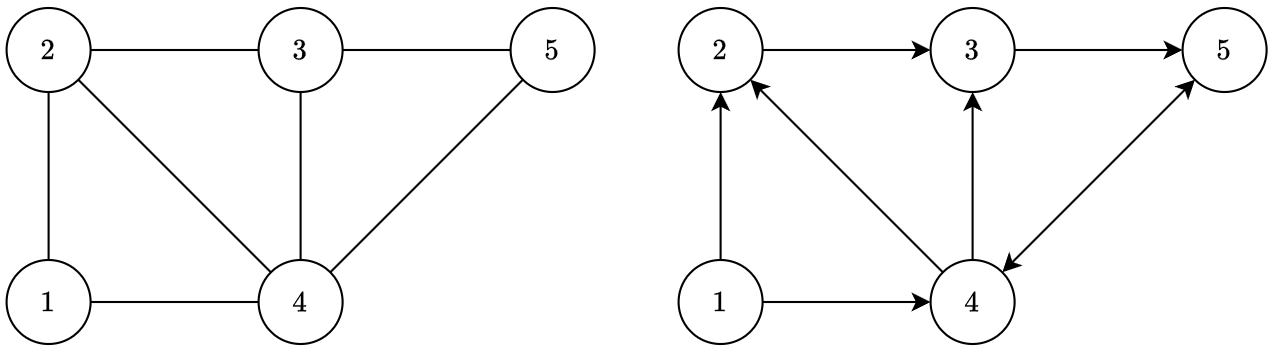
\includegraphics[width=0.75\linewidth]{images/graph.png}
        \end{figure}
    \end{example}
    \begin{definition}
        A \emph{directed path from $i \in N$ to $j \in N$} is a sequence of arcs $p=\langle \{v_1,v_2\},\{v_2,v_3\},\dots,\{v_{k-1},v_k\}\rangle $ connecting nodes $v_1$ and $v_k$.

        Nodes $u$ and $v$ are \emph{connected} if there is a path connecting them. A graph $(N,E)$ is connected if $u,v$ are connected for any $u,v \in N$. 
        
        A graph is \emph{strongly connected} if $u,v$ are connected by a directed path for any $u,v \in N$. 
        
        A \emph{cycle} or circuit is a path with $v_1=v_k$.
    \end{definition}
    \begin{example}
        The undirected graph has a path $\langle \{2,3\},\{3,4\},\{4,5\}\rangle$ from node $2$ to node $5$. So we say those nodes are connected. 
        
        The directed graph has a directed path $\langle (3,5),(5,4),(4,2),(2,3),(3,4) \rangle$ from node $3$ to node $4$. So we say those nodes are not strongly connected. 
        
        In the undirected graph $\langle \{2,3\},\{3,5\},\{5,4\},\{4,2\}\rangle$ is a cycle. 
        In the directed graph $\langle (2,3),(3,4),(4,2) \rangle$ is a circuit. 
        \begin{figure}[H]
            \centering
            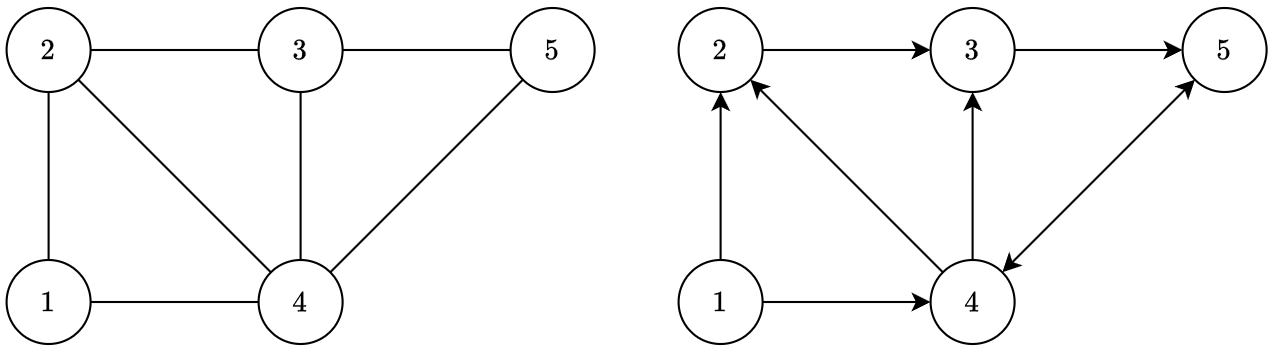
\includegraphics[width=0.75\linewidth]{images/graph.png}
        \end{figure}
    \end{example}
    \begin{definition}
        A graph is \emph{bipartite} if there is a partition $N=N_1 \cup N_2$ with $N_1 \cap N_1 = \varnothing$ such that no edge connects nodes in the same subset. 

        A graph is \emph{complete} if $E=\{ \{v_i,v_j\} | v_i,v_j \in N \land i \leq j \}$
    \end{definition}
    \begin{example}
        The graphic on the left is bipartite because we can find two subsets of nodes such that $N=N_1 \cup N_2$ with $N_1 \cap N_1 = \varnothing$ that are: $N_1=\{1,2,3\}$ and 
        $N_2=\{4,5\}$. The graph on the right is a complete graph because all the nodes are connected with each other. 
        \begin{figure}[H]
            \centering
            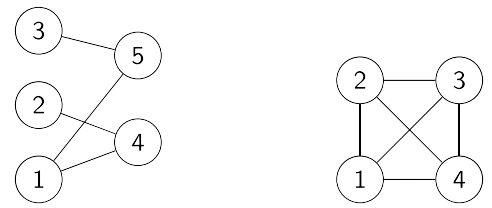
\includegraphics[width=0.5\linewidth]{images/bipcomp.png}
        \end{figure}
    \end{example}
    \begin{definition}
        Given a directed graph $G=(N,A)$ and $S \subset NM$, the \emph{outgoing cut} induced by $S$ is:
        \[ \delta^{+}(S)=\{(u,v) \in A | u \in S \land v \in N-S \} \]

        Given a directed graph $G=(N,A)$ and $S \subset NM$, the \emph{incoming cut} induced by $S$ is:
        \[ \delta^{-}(S)=\{(u,v) \in A | v \in S \land u \in N-S \} \]
    \end{definition}
    \begin{example}
        In the following graph we can note that: 
        \begin{itemize}
            \item $\delta^{+}(\{1,4\})=\{(1,2),(4,2),(4,5)\}$
            \item $\delta^{-}(\{1,4\})=\{(3,4),(5,4)\}$
        \end{itemize}
        \begin{figure}[H]
            \centering
            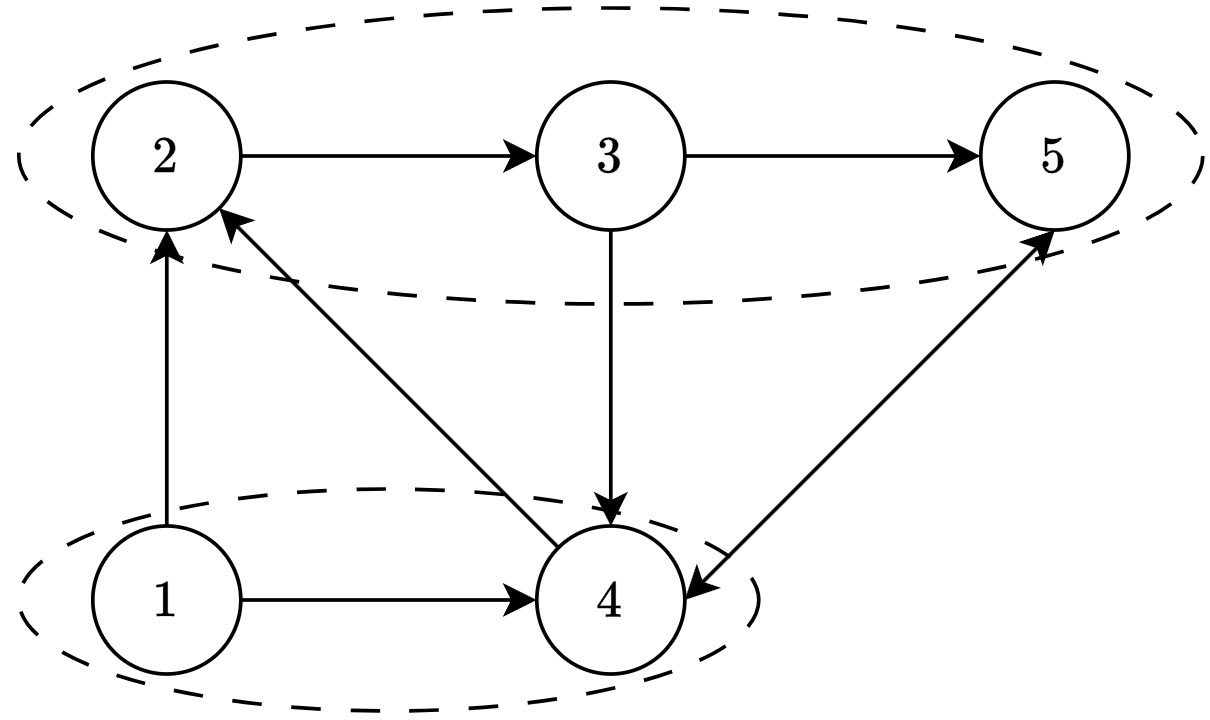
\includegraphics[width=0.75\linewidth]{images/cuts.png}
        \end{figure}
    \end{example}
    An undirected graph with $n$ nodes has at most $m=n(n-1)$ arcs. 
    A directed graph with $n$ nodes has at most $m=\dfrac{n(n-1)}{2}$ arcs.
    \begin{definition}
        Given $m$, the number of arcs or edges, and $n$, the number of nodes of the graph, we have that a graph is called \emph{dense} if:
        \[m \approx n^2\]

        Given $m$, the number of arcs or edges, and $n$, the number of nodes of the graph, we have that a graph is called \emph{sparse} if:
        \[m \ll n^2\]
    \end{definition}
    The best way to represent a dense graph is by using an $n \times n$ adjacency matrix, that is defined in the following way: 
    \[
    \begin{cases}
        a_{ij}=1 \:\:\:\:\:\: \textnormal{if}\:(i,j) \in A \\
        a_{ij}=0 \:\:\:\:\:\: \textnormal{otherwise}    
    \end{cases}    
    \]
    The best way to represent a sparse graph is by using lists of successors for each node. 
    \begin{example}
        The adjacency matrix for the following graph is: 
        \[A=
        \begin{bmatrix}
            0 & 1 & 0 & 1 & 0 \\
            0 & 0 & 1 & 0 & 0 \\
            0 & 0 & 0 & 1 & 1 \\
            0 & 1 & 0 & 0 & 1 \\
            0 & 0 & 0 & 1 & 0 
            \end{bmatrix}
        \]
        And the list of successor is: 
        \[S(1)=\{2,4\} \:\:\: S(2)=\{3\} \:\:\:S(3)=\{4,5\} \:\:\: S(4)=\{2,5\} \:\:\: S(5)=\{4\} \:\:\:\]
        \begin{figure}[H]
            \centering
            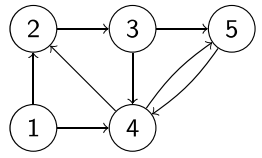
\includegraphics[width=0.3\linewidth]{images/graphs.png}
        \end{figure}
    \end{example}
    \begin{definition}
        $G^{'}=(N^{'},E^{'})$ is a \emph{sub-graph} of $G=(N,E)$ if $N^{'} \subseteq N$ and $E^{'} \subseteq E$. 

        A \emph{tree} $G_T=(N^{'},T)$ \emph{of $G$} is a connected and acyclic sub-graph of $G$. 

        $G_T=(N^{'},T)$ is a \emph{spanning tree of $G$} if it contains all nodes in $G$. 

        The \emph{leaves} of a tree are the nodes of degree one. 
    \end{definition}
    \begin{example}
        Given the following graph: 
        \begin{figure}[H]
            \centering
            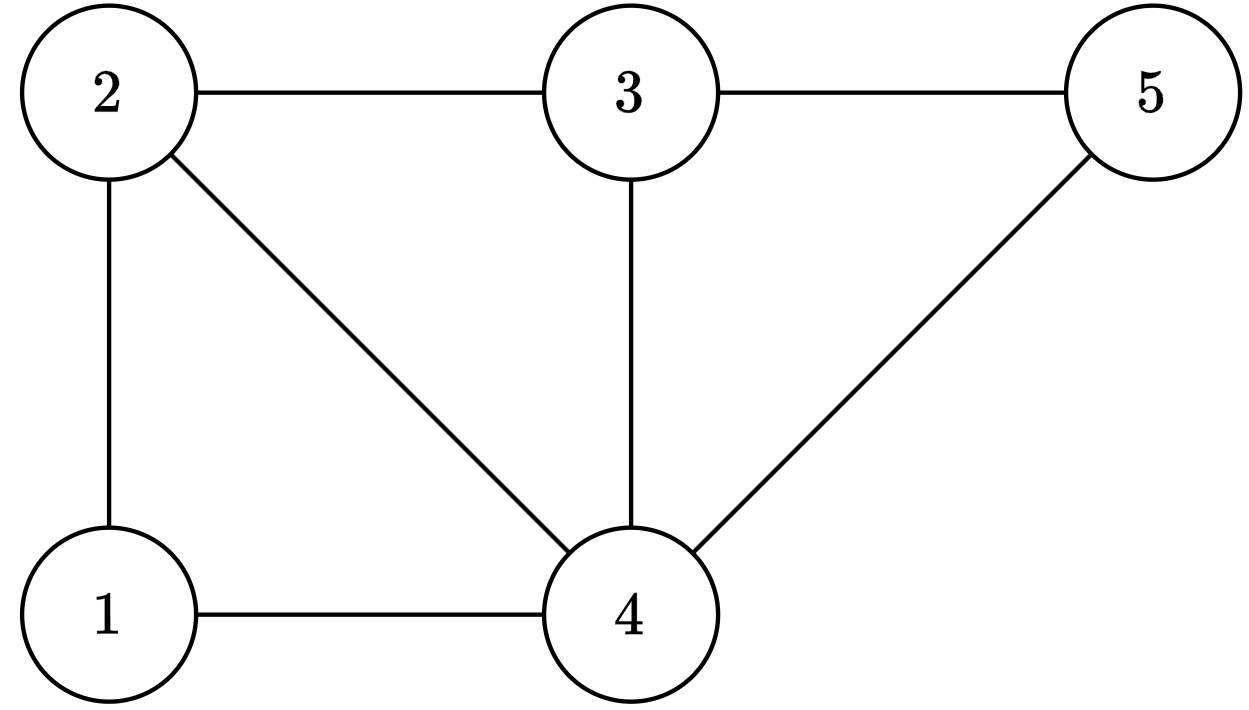
\includegraphics[width=0.3\linewidth]{images/sgraph.png}
        \end{figure}
        We can obtain: a sub-graph, a tree, and a spanning tree: 
        \begin{figure}[H]
            \centering
            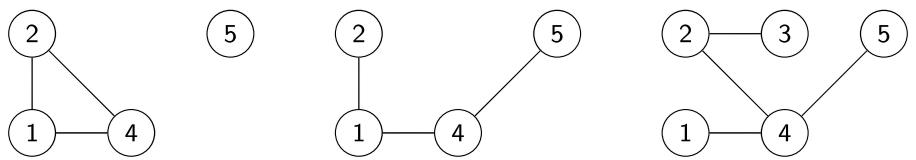
\includegraphics[width=0.8\linewidth]{images/sgraphmod.png}
        \end{figure}
    \end{example}
    The trees have the following properties: 
    \begin{enumerate}
        \item Every tree with $n$ nodes has $n-1$ edges. 
        \item Any pair of nodes in a tree is connected via a unique path. 
        \item By adding a new edge to a tree, we create a unique cycle. 
        \item Let $G_T=(N,T)$ be a spanning tree of $G=(N,E)$. Consider an edge $e \notin T$ and the unique cycle $C$ of $T \cup \{e\}$. For each edge $f \in C-\{e\}$, the 
            sub-graph $T\cup \{e\}-\{f\}$ is also a spanning tree of $G$. 
        \item Let $F$ be a partial tree contained in an optimal tree of $G$. Consider $e\{u,v\}\in \delta(S)$ of minimum cost, then there exists a minimum cost spanning tree of 
            $G$ containing $e$. 
        \item If $c_j \geq 0$ for all $(i,j) \in A$, there is at least one shortest path which is simple. 
        \item The directed graph G representing any project is acyclic (it is a DAG). 
        \item The minimum overall project duration is the length of the longest path from $s$ to $t$. 
        \item Given a feasible flow $x$ from $s$ to $t$, for each cut $\delta(S)$ separating $s$ from $t$, we have $\varphi(S)=\varphi(\{s\})$.
        \item For every feasible flow $x$ from $s$ to $t$ and every cut $\delta(S)$, with $S \subseteq V$, separating $s$ from $t$, we have $\varphi(S) \leq k(S)$. In other words,
            the value of the flow is less or equal to the capacity of the cut. 
    \end{enumerate}
    \begin{proof}[Property one]
        We will demonstrate this property with a proof by induction. For the base case we have that the claim holds for $n=1$. 
        For the inductive step we have to show that, if this is true for trees with $n$ nodes, then it is also true for those with $n+1$ nodes. 
        Let $T_1$ be a tree with $n+1$ nodes and recall that any tree with $n \geq 2$ nodes has at least two leaves. By deleting one of the leaf and its incident edge we obtain
        a tree $T_2$ with $n$ nodes. By induction hypothesis, $T_2$ has $n-1$ edges. Therefore, the tree $T_1$ has $n-1+1=n$ edges. 
    \end{proof}
    \begin{proof}[Property five]
        By contradiction, assume $T^{*} \subseteq E$ is a minimum cost spanning tree with $F \subseteq T^{*}$ and $e \notin T^{*}$. Adding edge $e$ to $T^{*}$ creates the cycle
        $C$. Let $f \in \delta(S) \cap C$: 
        \begin{itemize}
            \item If $c_e=c_f$, then $T^{*}\cup\{e\}-\{f\}$ is also optimal since it has same cost of $T^{*}$.
            \item If $c_e<c_f$, then $c\left(T^{*}\cup\{e\}-\{f\}\right)<C(T^{*})$, hence $T^{*}$ is not optimal.
        \end{itemize}
    \end{proof}
    \begin{proof}[Property seven]
        By contradiction, if $A_{i1} \varpropto A_{12},\dots,A_{jk} \varpropto A_{ki}$ there would be a logical inconsistency. 
    \end{proof}  
    \begin{proof}[Property eight]
        Since any $s-t$ path represents a sequence of activities that must be executed in the specified order, its length provides a lower bound on the minimum overall
        project duration. 
    \end{proof}  
    \begin{proof}[Property ten]
        By the definition of value of the flow through the cut $\delta(S)$ we have:
        \[\varphi(S)=\sum_{(i,j) \in \delta^{+}(S)}x_{ij}-\sum_{(i,j) \in \delta^{-}(S)}x_{ij}\]
        and because $0 \leq x_{ij } \leq k_{ij}$, for any $(i, j) \in A$ we also have
        \[\sum_{(i,j) \in \delta^{+}(S)}x_{ij}-\sum_{(i,j) \in \delta^{-}(S)}x_{ij} \leq \sum_{(i,j) \in \delta^{+}(S)}k_{ij}=k(S)\]
        Then, $\varphi(S) \leq k(S)$.
    \end{proof}  

    \section{Graph reachability problem}
    Given the directed graph $G=(N,A)$ and a node $s$, determine all the nodes that are reachable from $s$. 
    \begin{algorithm}[H]
        \caption{Graph reachability problem}
            \begin{algorithmic}[1]
                \State $Q \leftarrow \{s\}$
                \State $M \leftarrow \{\varnothing\}$
                \While {$Q \neq 0$}
                    \State $u \leftarrow \textnormal{node in } Q$
                    \State $Q \leftarrow Q-\{u\}$
                    \State $M \leftarrow M \cup \{u\}$
                    \For {$(u,v) \in \delta^{+}(u)$}
                        \If {$v \notin M$ and $v \notin Q$}
                            \State $Q \leftarrow Q \cup \{v\}$
                        \EndIf
                    \EndFor
                \EndWhile
            \end{algorithmic}
    \end{algorithm}
    The worst case complexity of the previous algorithm is $O(n^2)$.
    \begin{example}
        Given the following graph and $s=2$ the algorithm makes the following steps: 
        \begin{enumerate}
            \item $Q=\{2\} \:\:\:\:\:\:\:\:\:\:\: M=\varnothing$
            \item $Q=\{3\} \:\:\:\:\:\:\:\:\:\:\: M=\{2\}$
            \item $Q=\{4,5\} \:\:\:\:\:\:\: M=\{2,3\}$
            \item $Q=\{5\} \:\:\:\:\:\:\:\:\:\:\: M=\{2,3,4\}$
            \item $Q=\varnothing \:\:\:\:\:\:\:\:\:\:\:\:\:\: M=\{2,3,4,5\}$
        \end{enumerate}
        So the nodes $\{2,3,4,5\}$ are reachable from node two. 
        \begin{figure}[H]
            \centering
            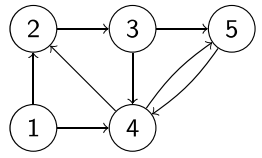
\includegraphics[width=0.3\linewidth]{images/graphs.png}
        \end{figure}
    \end{example}

    \section{Minimum spanning tree problem}
    Given an undirected graph $G=(N,E)$ and a cost function, find a spanning tree $G_T=(N,T)$ of minimum total cost: 
    \[\min_{T \in X} \sum_{e \in T}c_e\]
    where $X$ is the set of all spanning trees of $G$. 
    \begin{theorem}[Cayley]
        A complete graph with $n$ nodes $(n \geq 1)$ has $n^{(n-2)}$ spanning trees. 
    \end{theorem}
    To find the spanning tree with the minimum total cost we can use an algorithm that iteratively builds the spanning tree. The algorithm for the minimum spanning tree problem
    is the following: 
    \begin{enumerate}
        \item Select any node arbitrarily, and connect it to the nearest distinct node.
        \item Identify the unconnected node that is closest to a connected node, and then connect these two nodes. Repeat this step until all nodes have been connected.
    \end{enumerate}
    \begin{example}
        Apply the Prim's algorithm to the following graph: 
        \begin{figure}[H]
            \centering
            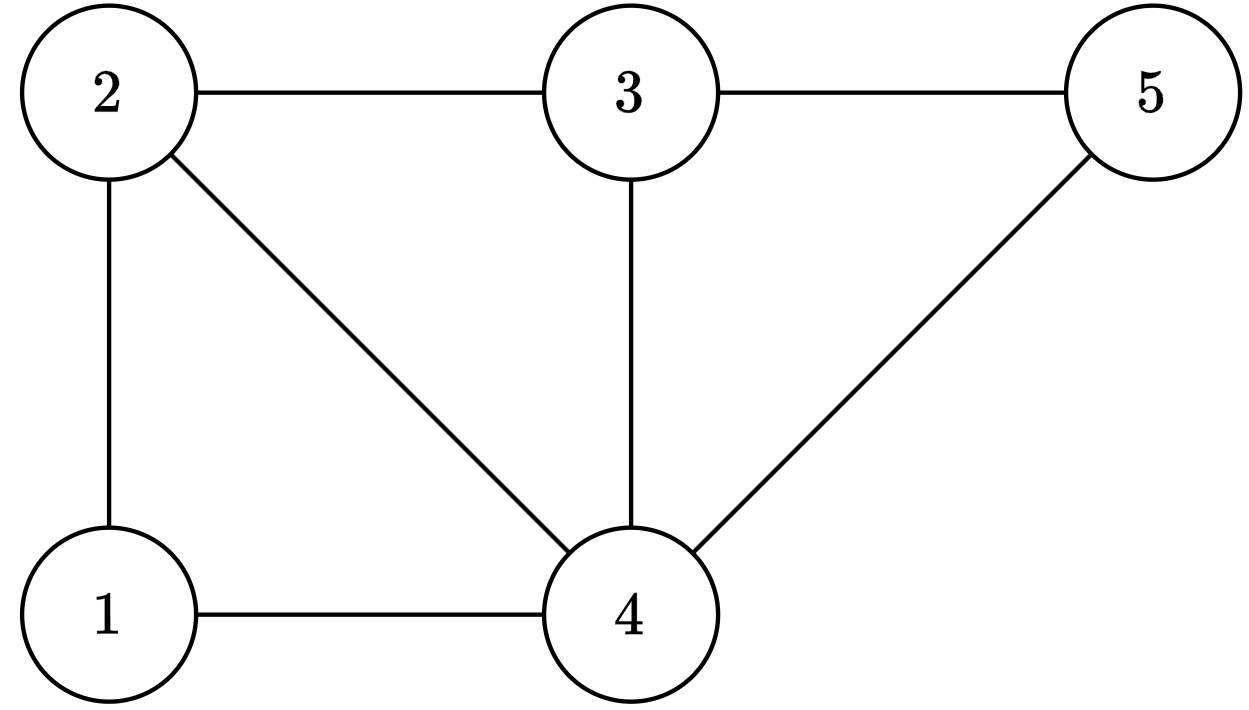
\includegraphics[width=0.3\linewidth]{images/sgraph.png}
        \end{figure}
        We select the node $3$ as starting node, and so we have $S=\{3\} \: T=\{\varnothing\}$, then:
        \begin{itemize}
            \item The edge with minimum cost is the one that connects the nodes $3$ and $4$. Now we have: $S=\{3,4\}$ and $T=\{\{3,4\}\}$.
            \item The edge with minimum cost is the one that connects the nodes $1$ and $4$. Now we have: $S=\{1,3,4\}$ and $T=\{\{3,4\},\{1,4\}\}$.
            \item The edge with minimum cost is the one that connects the nodes $4$ and $5$. Now we have: $S=\{1,3,4,5\}$ and $T=\{\{3,4\},\{1,4\},\{4,5\}\}$.
            \item The edge with minimum cost is the one that connects the nodes $4$ and $5$. Now we have: $S=N$ and $T=\{\{3,4\},\{1,4\},\{4,5\},\{2,4\}\}$.
        \end{itemize}
        The total cost in this case is equal to $c(T)=6$. Graphically, we have the following graphs: 
        \begin{figure}[H]
            \centering
            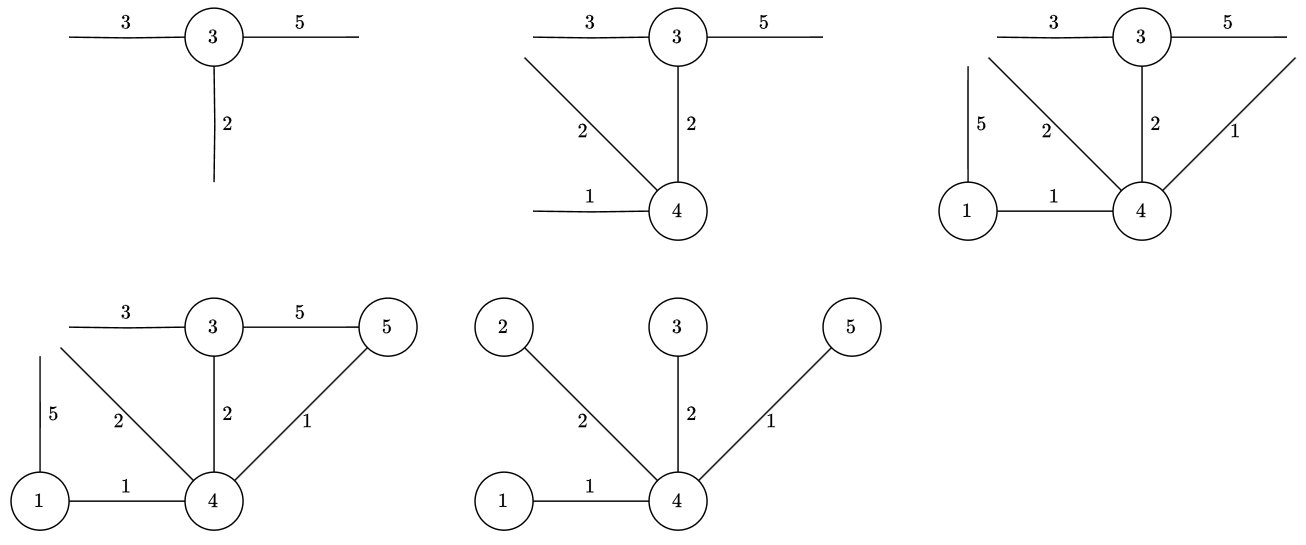
\includegraphics[width=0.75\linewidth]{images/MST.png}
        \end{figure}
    \end{example}
    Given a connected graph $G=(N,E)$ with edge cost the algorithm outputs $T \subseteq N$ of edges of $G$ such that $G_T=(N,T)$ is a minimum cost spanning tree of $G$. 
    \begin{algorithm}[H]
        \caption{Prim's algorithm for the minimum cost spanning tree problem}
            \begin{algorithmic}[1]
                \State $S \leftarrow \{u\}$
                \State $T \leftarrow \{\varnothing\}$
                \While {$\left\lvert T \right\rvert < n-1$}
                    \State $\{u,v\}\leftarrow \textnormal{edge in} \delta(S) \textnormal{of minimum cost}$
                    \State $S \leftarrow S \cup \{v\}$
                    \State $T \leftarrow T \cup \{u,v\}$
                \EndWhile
            \end{algorithmic}
    \end{algorithm}
    where $u \in S$ and $v \in N-S$. The worst-case complexity is $O(n^2)$. 
    \begin{example}[Proposition]
        Prim's algorithm is exact. 
    \end{example}        
    The exactness does not depend on the choice of the first node nor on the selected edge of minimum cost in $\delta(S)$. 
    \begin{example}[Proposition]
        Prim's algorithm is greedy. 
    \end{example}     
    At each step a minimum cost edge is selected among those in the cut $\delta (S)$ induced by the current set of nodes $S$. 
    \begin{definition}
        Given a spanning tree $T$, an edge $e \notin T$ is \emph{cost decreasing} if when $e$ is added to $T$ it creates a cycle $C$ with $C \subseteq T \cup \{e\}$ and 
        $\exists f \in C-\{e\}$ such that $c_e<c_f$. 
    \end{definition}
    \begin{example}
        Given the following graph
        \begin{figure}[H]
            \centering
            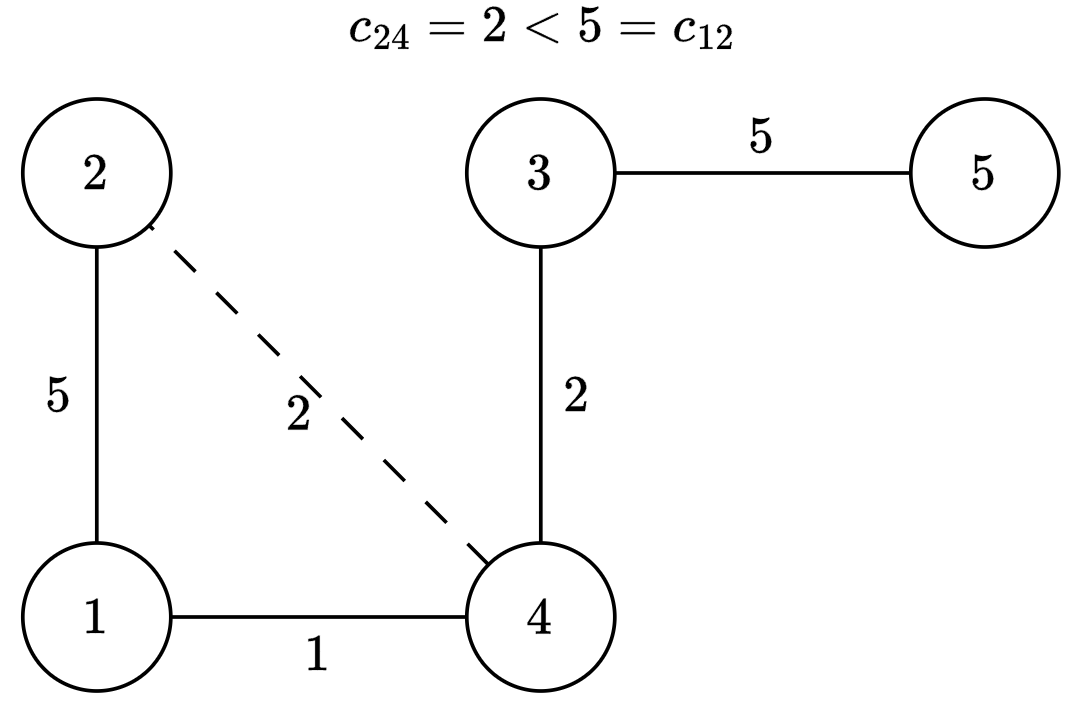
\includegraphics[width=0.5\linewidth]{images/costdecreasing.png}
        \end{figure}
        Because $c(T \cup \{e\}-\{f\})=c(T)+c_e-c_f$, if $e$ is cost decreasing, then
        \[c(T \cup \{e\}-\{f\})<c(T)\]
    \end{example}
    \begin{theorem}[Tree optimaility condition]
        A tree $T$ is of minimum total cost if and only if no cost decreasing edge exists. 
    \end{theorem}
    \begin{proof}[of direct implication]
        If a cost-decreasing edge exists, then T is not of minimum total cost.
    \end{proof}
    \begin{proof}[of inverse implication]
        If no cost-decreasing edge exists, then $T$ is of minimum total cost. Let $T^{*}$ be a minimum cost spanning tree found by Prim's algorithm. It can be verified that, by 
        exchanging one edge at a time, $T^{*}$ can be iteratively transformed into $T$ without modifying the total cost. Thus, $T$ is also optimal. 
    \end{proof}
    The optimality condition allows us to verify whether a spanning tree $T$ is optimal: it is sufficient to check that each $e \in E-T$ is not a cost-decreasing edge. 

    \section{Graph shortest path problem}
    \subsection{Dijkstra's algorithm}
    Given a directed graph $G=(N,A)$ with a cost $c_j \in R$ for each arc $(i,j) \in A$, and two nodes $s$ and $t$, determine a minimum cost path from $s$ to $t$. 

    Each value $c_j$ represents the cost  of arc $(i,j) \in A$. Node $s$ is the origin, or source, and $t$ is the destination, or sink. 
    \begin{definition}
        A path is \emph{simple} if no node is visited more than once. 
    \end{definition}
    The input of Dijkstra's algorithm is a graph $G = (N, A)$ with non-negative arc costs and $s \in N$. This algorithm will give us the shortest paths from $s$ to 
    all other nodes of $G$. The idea behind it is to consider the nodes in increasing order of cost of the shortest path from $s$ to any one of the other nodes. 
    To each node $j \in N$, we assign a label $L_j$ which corresponds to the cost of a minimum cost path from $s$ to $j$ and a label $pred_j$ that is the predecessor of $j$ in the
    shortest path from $s$ to $j$. Note that this algorithm is greedy with respect to path from $s$ to $j$. 
    \begin{example}
        Given a graph, and selecting $1$ as the initial node, we set the following labels.
        \begin{figure}[H]
            \centering
            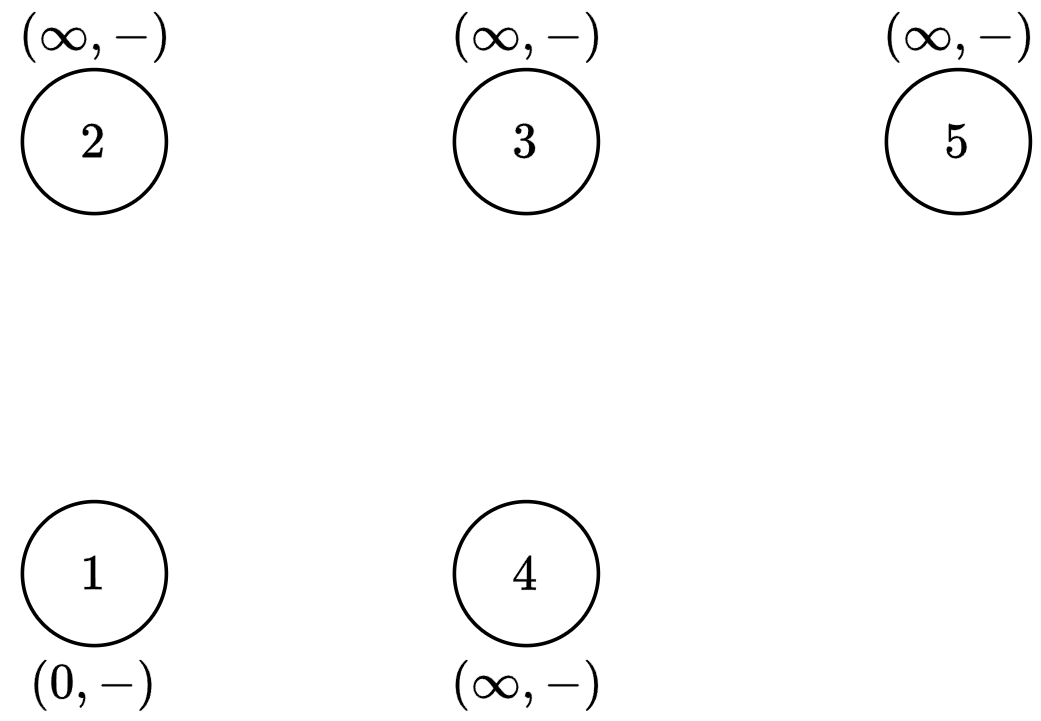
\includegraphics[width=0.25\linewidth]{images/D1.png}
        \end{figure}
        Next, we check all the arcs going from the starting node to other nodes, and we update the nodes label (the node one will always have no predecessor and null cost).
        \begin{figure}[H]
            \centering
            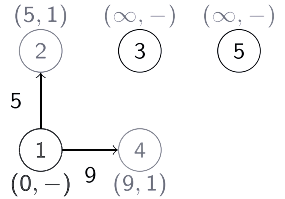
\includegraphics[width=0.25\linewidth]{images/D2.png}
        \end{figure}
        Now, we move to the node $2$ and check all the reachable nodes. In this case we found the shortest path from the initial node to $4$, so we update the label of $4$.
        \begin{figure}[H]
            \centering
            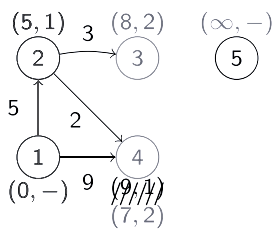
\includegraphics[width=0.25\linewidth]{images/D3.png}
        \end{figure}
        Now, we move to the node $4$ that is the closest node to $s$, and we check all the arcs going in other nodes.
        \begin{figure}[H]
            \centering
            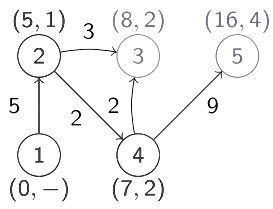
\includegraphics[width=0.25\linewidth]{images/D4.png}
        \end{figure}
        We do the same for the remaining nodes, again in increasing order of cost from the start. 
        \begin{figure}[H]
            \centering
            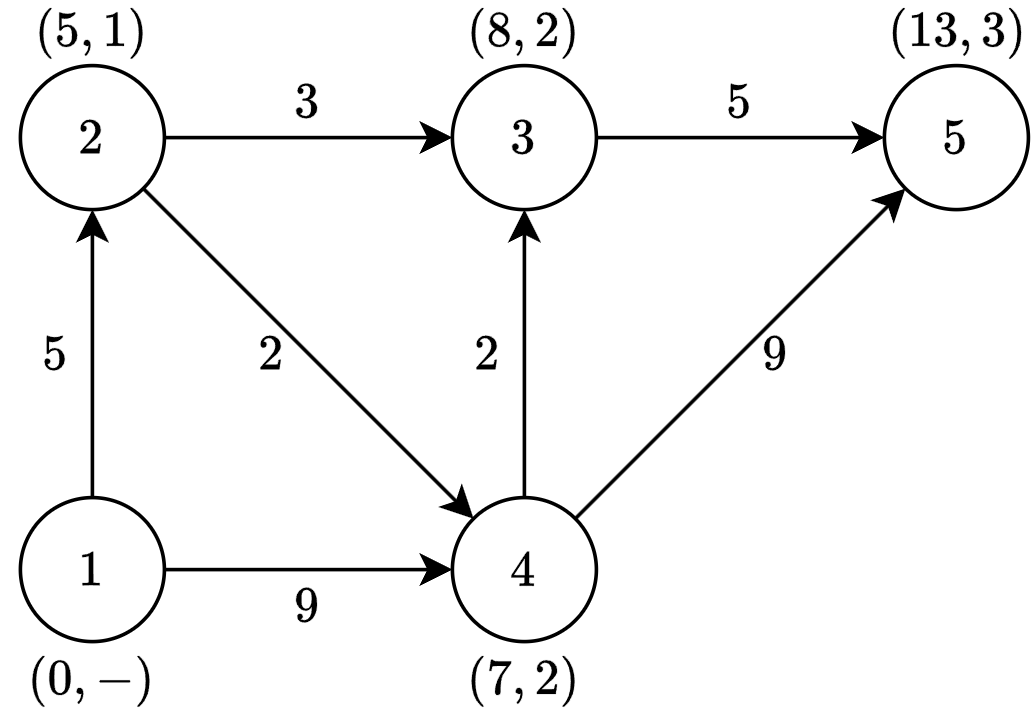
\includegraphics[width=0.5\linewidth]{images/D5.png}
        \end{figure}
        It is now possible to retrieve backward the shortest path to any node of the graph using the predecessor label. For instance, we have that the shortest path from $s$ to $5$
        has a cost of $13$ and the path is $(1,2,3,5)$. 
    \end{example}

    The inputs of the algorithm are: a graph $G = (N, E)$ with non-negative arc costs, $s \in N$. 
    \begin{algorithm}[H]
        \caption{Dijkstra's algorithm for the graph shortest path problem}
            \begin{algorithmic}[1]
                \State $S \leftarrow \varnothing$
                \State $X \leftarrow \{s\}$
                \For {$u \in N$}
                    \State $L_u \leftarrow +\infty$
                \EndFor
                \State $L_s \leftarrow 0$
                \While {$\left\lvert S \right\rvert \neq n$}
                    \State $u \leftarrow \textnormal{argmin}\{L_i|i \in X\}$
                    \State $X \leftarrow X-\{u\}$
                    \State $S \leftarrow S \cup \{u\}$
                    \For {$(u,v) \in \delta^{+}(u) \: \textnormal{such that} \: L_v> L_u + c_{uv} $}
                        \State $L_v \leftarrow L_u+c_{uv}$
                        \State $pred_v \leftarrow u$
                        \State $X \leftarrow X \cup \{v\}$
                    \EndFor
                \EndWhile
            \end{algorithmic}
    \end{algorithm}
    The worst case complexity of this algorithm is $O(n^3)$. 
    \begin{example}[Proposition]
        Dijkstra's algorithm is exact. 
    \end{example}
    \begin{proof}
        At the $k$-th step: $S = \{s,i_2,\dots,i_k\}$ and 
        \[L_j=
        \begin{cases}
            \textnormal{cost of a minimum path from } s \textnormal{ to } j,\:j \in S \\ 
            \textnormal{cost of a minimum path with all intermediate nodes in } S, \: j \notin S
        \end{cases}
        \]
        By induction on the number $k$ of steps: 
        \begin{itemize}
            \item Base case: it is easy to see that the statement holds for $k = 1$, since 
                \[S=\{s\},\: L_s=0,\: L_j= +\infty,\: \forall j \neq S \]
            \item Inductive step: we must prove that, if the statement holds at the $k$-th step, it must also hold for the $(k + 1)$-th step. 
        \end{itemize}
        In the $(k + 1)$-th step let $u \notin S$be the node that is inserted in $S$ and $\varnothing$ the path from $s$ to $u$ such that:
        \[L_v + c_{uv} \leq L_i + C_{ij},\: \forall(i,j) \in \delta^{+}(S)\]
        Let us verify that every path $\pi$ from $s$ to $u$ has $c(\pi) \geq c(\varnothing)$. There exist $i \in S$ and $j \notin S$ such that: 
        \[\pi= \pi_1 \cup \{(i,j)\} \cup \pi_2\]
        Where $(i, j)$ is the first arc in $\pi \cap \delta^{+}(S)$. Moreover: 
        \[c(\pi) = c(\pi_1) + c_{ij} + c(\pi_2) \geq L_i + c_{ij}\]
        Because $c_{ij} \geq 0$, thus, $c(\pi_2) \geq 0$, and by the induction assumption, $c(\pi_1) \geq L_i$. Finally, by the choice of $(v,u)$ we have: 
        \[L_i + c_{ij} \geq L_v + c_{vu} = c(\varnothing)\]
    \end{proof}
    We can note that: 
    \begin{itemize}
        \item A set of the shortest paths from $s$ to all the nodes $j$ can be retrieved via the vector of predecessors. 
        \item The union of a set of the shortest paths from node $s$ to all the other nodes of $G$ is the shortest path trees rooted at $s$. Such shortest path trees have 
            nothing to do with minimum cost spanning trees. 
        \item Dijkstra's algorithm does not work when there are arcs with negative cost. 
    \end{itemize}

    \subsection{Floyd-Warshall's algorithm}
    If the graph $G$ contains a circuit of negative cost, the shortest path problem may not be well-defined. Each time the circuit appears, the cost decreases. There is no 
    finite shortest path from $s$ to $t$. Floyd-Warshall's algorithm detects the presence of circuits with negative cost. It provides a set of the shortest paths between all pairs
    of nodes, even when there are arcs with negative cost. It is based on iteratively applying a triangular operation. 
    The algorithm uses two $n \times n$ matrices, D, P, whose elements correspond, at the end of the algorithm to: 
    \begin{itemize}
        \item $d_{ij}$, that is the cost of the shortest path from $i$ to $j$.
        \item $p_{ij}$, that is the predecessor of $j$ in that shortest path from $i$ to $j$.
    \end{itemize}
    \begin{definition}
        The \emph{triangular operation} states that for each pair of nodes $i,j$ with $i \neq u$ and $j \neq u$ (including case $i=j$), check whether when going from $i$ to $j$ it is 
        more convenient to go via $u$, so if the following relation holds: 
        \[d_{iu}+d_{uj} < d_{ij}\]
    \end{definition}
    \begin{example}
        Given the following graph: 
        \begin{figure}[H]
            \centering
            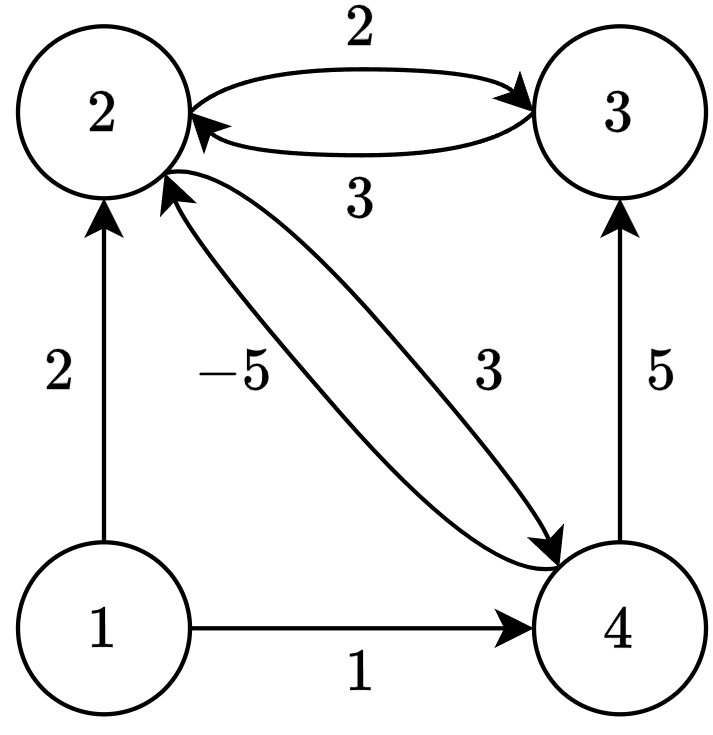
\includegraphics[width=0.25\linewidth]{images/floyd.png}
        \end{figure}
        We have to initialize the matrices in the following way: 
        \[D=\begin{bmatrix}
            0 & 2 & \infty & 1 \\
            \infty & 0 & 3 & 3 \\
            \infty & 2 & 0 & \infty \\
            \infty & -5 & 5 & 0 \\
        \end{bmatrix}
        \:\:\:\:\:\:
        P=\begin{bmatrix}
            1 & 1 & 1 & 1 \\
            2 & 2 & 2 & 2 \\
            3 & 3 & 3 & 3 \\
            4 & 4 & 4 & 4 \\
        \end{bmatrix}
        \]
        The first iteration with $u=1$ (we consider the first row and the first column) leave the matrices unchanged, in fact the triangular operation is always satisfied: 
        \begin{itemize}
            \item $0=d_{22} < d_{21} + d_{12} = \infty + 2$ (no changes). 
            \item $3=d_{23} < d_{21} + d_{13} = \infty + \infty$ (no changes). 
            \item $3=d_{24} < d_{21} + d_{14} = \infty + 1$ (no changes). 
            \item $2=d_{32} < d_{31} + d_{12} = \infty + 2$ (no changes). 
            \item $0=d_{33} < d_{31} + d_{13} = \infty + \infty$ (no changes). 
            \item $\infty=d_{34} < d_{31} + d_{14} = \infty + 1$ (no changes). 
            \item $-5=d_{42} < d_{41} + d_{12} = \infty + 2$ (no changes). 
            \item $5=d_{43} < d_{41} + d_{13} = \infty + \infty$ (no changes). 
            \item $0=d_{44} < d_{41} + d_{14} = \infty + 1$ (no changes). 
        \end{itemize}
        The second iteration with $u=2$ (we consider the second row and the second column) changes the matrices and halts the algorithm because of the negative arc found: 
        \begin{itemize}
            \item $0=d_{11} < d_{12} + d_{21} = 2 +\infty $ (no changes). 
            \item $\infty=d_{13} < d_{12} + d_{23} = 2+3$ ($p_{13} \leftarrow p_{23}$). 
            \item $1=d_{14} < d_{12} + d_{24} = 2+3$ (no changes). 
            \item $\infty=d_{31} < d_{32} + d_{21} = 2 + \infty$ (no changes). 
            \item $0=d_{33} < d_{32} + d_{23} = 2+3$ (no changes). 
            \item $\infty=d_{34} < d_{32} + d_{24} = 2+3$ ($p_{34} \leftarrow p_{24}$). 
            \item $\infty=d_{41} < d_{42} + d_{21} = 5 + \infty$ (no changes). 
            \item $5=d_{43} < d_{42} + d_{23} = -5+3$ ($p_{43} \leftarrow p_{23}$). 
            \item $0=d_{44} < d_{42} + d_{24} = -5+3$ (negative cost circuit found). 
        \end{itemize}
    \end{example}

    The inputs of the algorithm are: a directed graph $G = (N,A)$ with an $n \times n$ cost matrix, $C = [c_{ij}]$.
    \begin{algorithm}[H]
        \caption{Walshall-Floyd's algorithm}
            \begin{algorithmic}[1]
                \For {$i \in N$}
                    \For {$j \in N$}
                        \State $p_{ij} \leftarrow i$
                        \State $d_{ij} \leftarrow \begin{cases}
                            0 \:\:\:\:\:\:\:\:\:\:\: i = j \\
                            c_{ij} \:\:\:\:\:\:\:\:\: i \neq j \land (i,j) \in A \\
                            +\infty \:\:\:\:\:\: \textnormal{otherwise}
                        \end{cases}$
                    \EndFor
                \EndFor
                \For {$u \in N$}
                    \For {$i \in N-\{u\}$}
                        \For {$j \in N-\{u\}$}
                            \If {$d_{iu}+d_{uj} \ d_{ij}$}
                                \State $p_{ij} \leftarrow p_{uj}$
                                \State $d_{ij} \leftarrow d_{iu}+d_{uj}$
                            \EndIf
                        \EndFor
                    \EndFor
                    \For {$i \in N$}
                        \If {$d_{ii} < 0$}
                            \State \Return
                        \EndIf
                    \EndFor
                \EndFor
            \end{algorithmic}
    \end{algorithm}
    Since in the worst case the triangular operation is executed for all nodes $u$ and for each pair of nodes $i$ and $j$, the overall complexity is $O(n^3)$. 
    \begin{example}[Proposition]
        Floyd-Warshall's algorithm is exact. 
    \end{example}
    \begin{proof}
        Assume that the nodes of $G$ are numbered from $1$ to $n$. Verify that, if the node index order is followed, after the $u$-th cycle the value $d_{ij}$ (for any $i$ and $j$) corresponds to the cost of 
        the shortest path from $i$ to $j$ with only intermediate nodes in ${1,\dots,u}$. 
    \end{proof}

    \subsection{Topological order algorithm}
    Given a directed acyclic graph $G = (N,A)$ with a cost $c_ij \in \mathbb{R}$ for each $(i,j) \in A$, and nodes $s$ and $t$, determine the shortest (longest) path from $s$ to $t$. 
    The DAGs have the following property called topological order: the nodes of any directed acyclic graph $G$ can be ordered topologically, that is, indexed so that for each arc $(i,j) \in A$ we have $i < j$. 
    The topological order can be exploited in a very efficient dynamic programming algorithm to find shortest (or longest) paths in DAGs. Given $G = (N,A)$ represented via the lists of predecessors
    $\delta^{-}(v)$ and successors $\delta^{+}(v)$ for each node $v$ we have to follow these steps: 
    \begin{enumerate}
        \item Assign the smallest positive integer not yet assigned to a node $v \in N$ with $\delta^{-}(v)=\varnothing$. 
        \item Delete the node $v$ with all its incident arcs. 
        \item Go back to the point one until there are nodes in the current sub-graph. 
    \end{enumerate}
    The complexity of this algorithm is $O(m)$ where $m = \left\lvert A \right\rvert $, because each node/arc is considered at most once. 
    \begin{example}
        A graphical example of the algorithm is the following: 
        \begin{figure}[H]
            \centering
            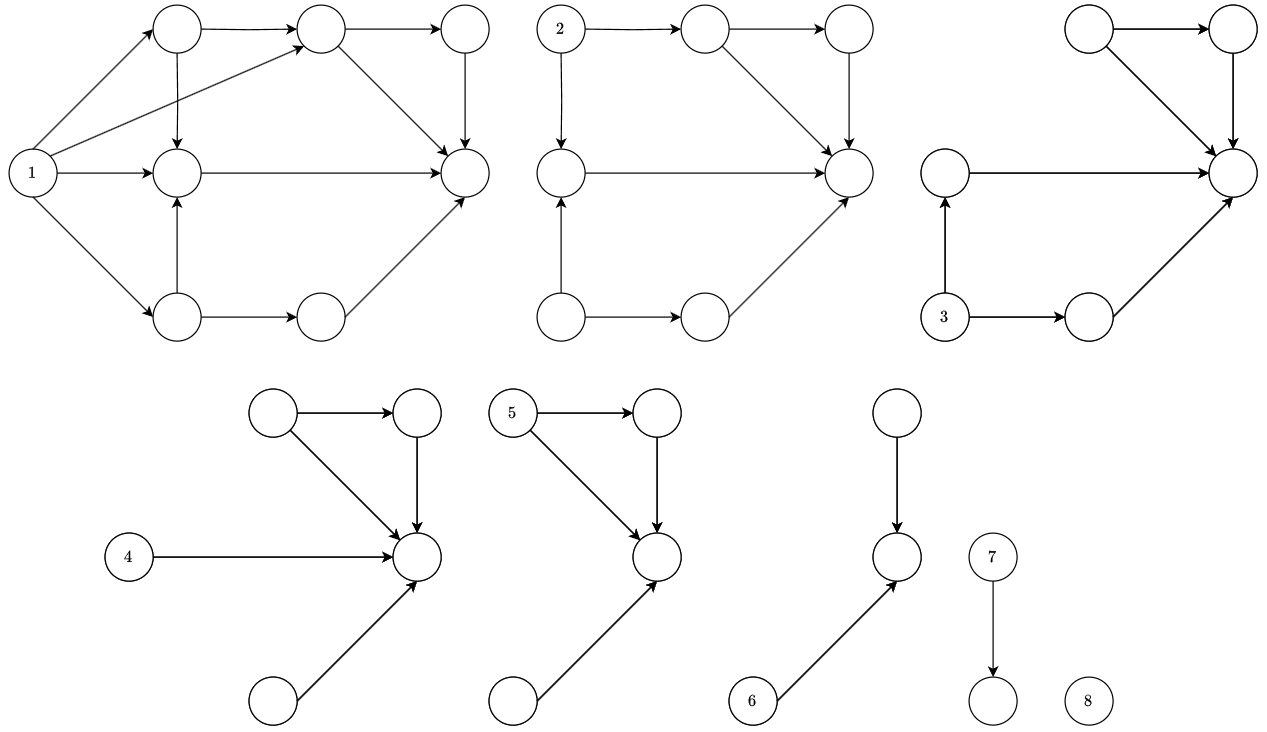
\includegraphics[width=0.8\linewidth]{images/spath.png}
        \end{figure}
    \end{example}

    \subsection{DAGs' dynamic programming algorithm}
    Any shortest path from 1 to $\pi_t$, with at least 2 arcs, can be subdivided into two parts: $\pi_t$ and $(i,t)$, where $\pi_t$ is the shortest sub-path from $s$ to $i$. 
    For each node  $i=1,\dots,t$, let $L_i$ be the cost of the shortest path from $1$ to $i$. Then: 
    \[L_t=\min_{(i,t) \in \delta^{-}(t)}\{L_i+c_{it}\}\]
    where the minimum is taken over all possible predecessors $i$ of $t$. If $G$ is directed, acyclic and topologically ordered, the only possible predecessors of $t$ in the shortest 
    path $\pi_t$ from $1$ to $t$ are those with index $i < t$. Thus,
    \[L_t=\min_{i<t}\{L_i+c_{it}\}\]
    In a graph with circuits, any node different from $t$ can be a predecessor of $t$ in $\pi_t$.  

    For DAGs whose nodes are topologically ordered $L_{t-1},\dots,_L1$ satisfy the same type of recursive relations:
    \[L_{t-1}=\min_{i<t-1}\{L_i+c_{i,t-1}\};\dots;L_2=\min_{i=1}\{L_i+c_i2\}=L_1+c_{12};L_1=0\]
    which can be solved in the reverse order:
    \[L_1=0;L_2=L_1+c_{12};\dots;L_{t}=\min_{i<t-1}\{L_i+c_{t}\}\]

    \begin{example}
        Given the following graph: 
        \begin{figure}[H]
            \centering
            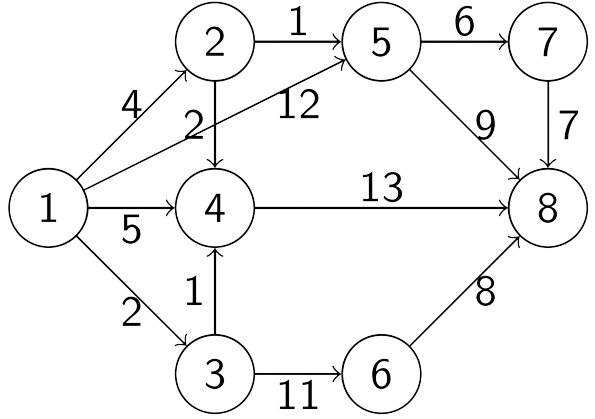
\includegraphics[width=0.5\linewidth]{images/DAG.png}
        \end{figure}
        The dynamic programming to find the shortest paths in DAGs follows this workflow: 
        \begin{itemize}
            \item $L_1=0 \rightarrow \textnormal{pred}_1=1$
            \item $L_2=L_1+c_{12}=4 \rightarrow \textnormal{pred}_2=1$
            \item $L_3=L_1+c_{13}=2 \rightarrow \textnormal{pred}_3=1$
            \item $L_4=\min_{i=1,2,3}\{L_i+c_{i4}\}=\min{5,6,3}=3 \rightarrow \textnormal{pred}_4=3$
            \item $L_5=\min_{i=1,2}\{L_i+c_{i5}\}=\min{12,5}=5 \rightarrow \textnormal{pred}_5=2$
            \item $L_6=L_3+c_{36}=13 \rightarrow \textnormal{pred}_6=3$
            \item $L_7=L_5+c_{57}=11 \rightarrow \textnormal{pred}_7=5$
            \item $L_8=\min_{i=4,5,6,7}\{L_i+c_{i8}\}=\min{16,14,21,18}=14 \rightarrow \textnormal{pred}_8=5$
        \end{itemize}
    \end{example}
    \begin{algorithm}[H]
        \caption{Dynamic programming to find the shortest paths in DAGs}
            \begin{algorithmic}[1]
                \State Sort the nodes of $G$ topologically
                \State $L_1 \leftarrow 0$
                \For {$j=2,\dots,n$}
                    \State $L_j \leftarrow \min\{L_i+c_{ij}|(i,j) \in \delta^{-}(j) \land i < j\}$
                    \State $pred_j \leftarrow v \: \textnormal{such that} \: (v,j)=\textnormal{argmin} \{L_i+c_{ij}|(i,j) \in \delta^{-}(j) \land i < j\}$
                \EndFor
            \end{algorithmic}
    \end{algorithm}
    Since the nodes are topologically ordered each node and each arc is considered exactly once, so we have a complexity of $O(m)$, where $m=\left\lvert A \right\rvert$. 
    
    It is possible to use the same algorithm to find the longest path with the formula: 
    \[L_t=\max_{i<t}\{L_i+c_{it}\},\dots\]

    \begin{example}[Proposition]
        The Dynamic Programming algorithm for DAGs is exact. 
    \end{example}
    \begin{proof}
        This is due to the optimality principle: for any shortest (longest) path from 1 to $t,\pi_t$, there exists $i < j$ such that the path can be subdivided into two parts: 
        $\pi_i$ and $(i,t)$, where $\pi_i$ is a minimum (maximum) length from $s$ to $i$. 
    \end{proof}

    \subsection{Project planning algorithm}
    \begin{definition}
        A \emph{project} consists of a set of $m$ activities with their duration: activity $A_i$ has an estimated duration $d_j \geq 0, i=1,\dots,m$. 

        Some pairs of activities are subject to a \emph{precedence constraint}: $A_i \varpropto A_j$  indicates that $A_j$ can start only after the end of $A_i$. 
    \end{definition}
    A project can be represented by a directed graph $G = (N, A)$ where each arc corresponds to an activity, and its arc length represents the duration of the corresponding 
    activity. To account for the precedence constraints, the arcs must be positioned so that 
    \[A_i \varpropto A_j\]
    implies that there exists a directed path where the arc associated to $A_i$ precedes the arc associated to $A_j$. Therefore, a node $v$ marks an event corresponding to the end of 
    all the activities $(i,v) \in \delta^{-}(v)$ and, hence, the possible beginning of all those $(v,j) \in \delta^{+}(v)$. 
    We can also introduce new nodes so that graph $G$: 
    \begin{itemize}
        \item Contains a unique initial node $s$ corresponding to the event beginning of the project.
        \item Contains a unique final node $t$ corresponding to the event end of the project. 
        \item Does not contain multiple arcs (with same endpoints). 
    \end{itemize}

    \begin{example}
        A project can be defined in the following way: 
        \begin{figure}[H]
            \centering
            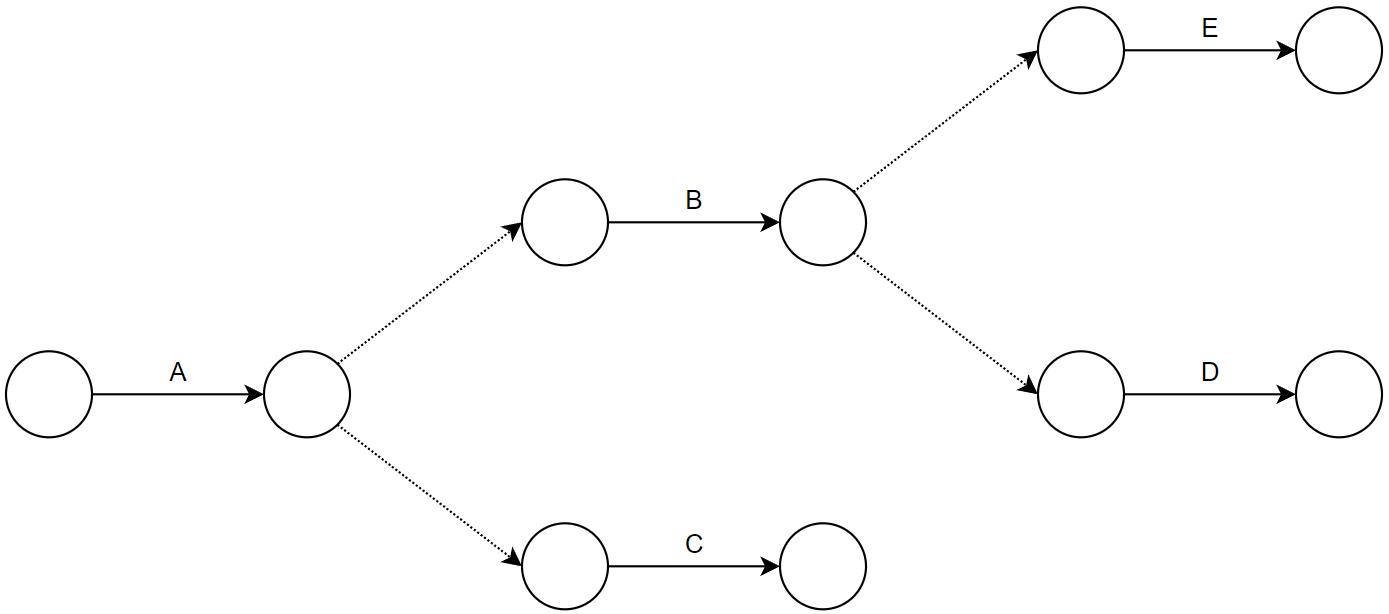
\includegraphics[width=0.8\linewidth]{images/project.png}
        \end{figure}
        This graph can be simplified by contracting some arcs, but we have to pay attention in introducing unwanted precedence constraints. The correct contracted graph is: 
        \begin{figure}[H]
            \centering
            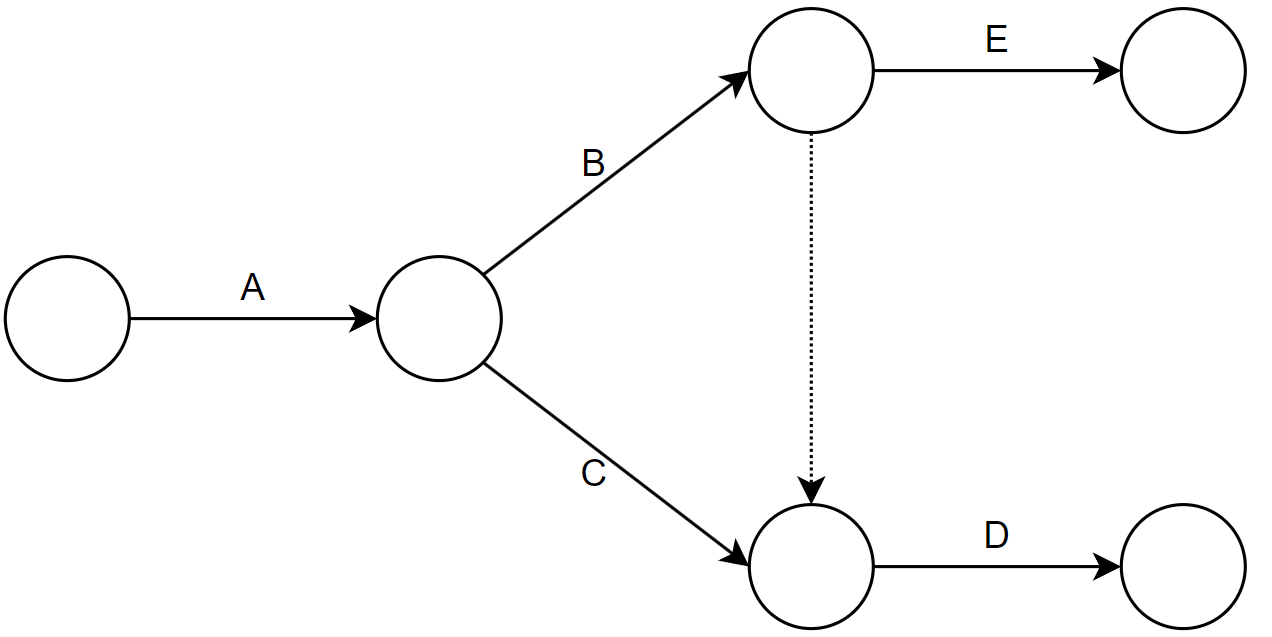
\includegraphics[width=0.4\linewidth]{images/cproject.png}
        \end{figure}
        We can add the initial and the final nodes: 
        \begin{figure}[H]
            \centering
            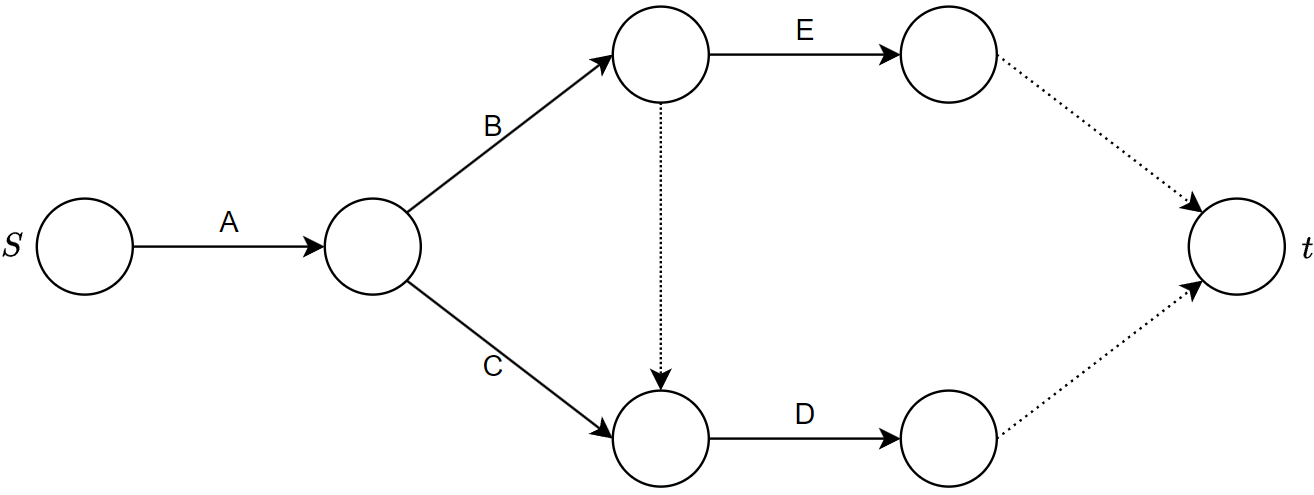
\includegraphics[width=0.5\linewidth]{images/fproject.png}
        \end{figure}
    \end{example}

    The problem to solve is: given a project, schedule the activities to minimize the overall project duration. To solve this problem with can use the critical path method that
    determines: 
    \begin{itemize}
        \item A schedule that minimizes the overall project duration. 
        \item The slack of each activity. 
    \end{itemize}
    The input of the algorithm is the graph $G$ representing the project and find a topological order of the nodes. The steps are: 
    \begin{enumerate}
        \item Consider the nodes by increasing indices and, for each $h \in N$, find the earliest time $T_{min_h}$ at which the event associated to node $h$ can occur
            ($T_{min_n}$ corresponds to the minimum project duration). 
        \item Consider the nodes by decreasing indices and, for each $h \in N$, find the latest time $T_{max_h}$, at which the event associated to node $h$ can occur
            without delaying the project completion date beyond $T_{min_n}$. 
        \item For each activity $(i,j) \in A$, find the slack: $\sigma_{ij}=T_{max_j}-T_{max_i}-d_{ij}$. 
    \end{enumerate}
    \begin{example}
        Consider the following project: 
        \begin{table}[H]
            \centering
            \begin{tabular}{ccc}
            \hline
            \textbf{Activity} & \textbf{Duration} & \textbf{Predecessors} \\ \hline
            A                 & 3                 & -                     \\
            B                 & 2                 & A                     \\
            C                 & 3                 & A                     \\
            D                 & 3                 & C                     \\
            E                 & 4                 & B,C                   \\
            F                 & 3                 & B                     \\
            G                 & 1                 & E,D                   \\
            H                 & 4                 & C                     \\
            I                 & 2                 & F                     \\ \hline
            \end{tabular}
        \end{table}
        With these precedence constraints: 
        \[A \varpropto B,A \varpropto C,C \varpropto D,B \varpropto E, C \varpropto E,B \varpropto F,E \varpropto G,D \varpropto G,C \varpropto H,F \varpropto I\]
        Determine the overall minimum duration of the project and the slack for each activity. We have to find the graph associated to the given problem, that is: 
        \begin{figure}[H]
            \centering
            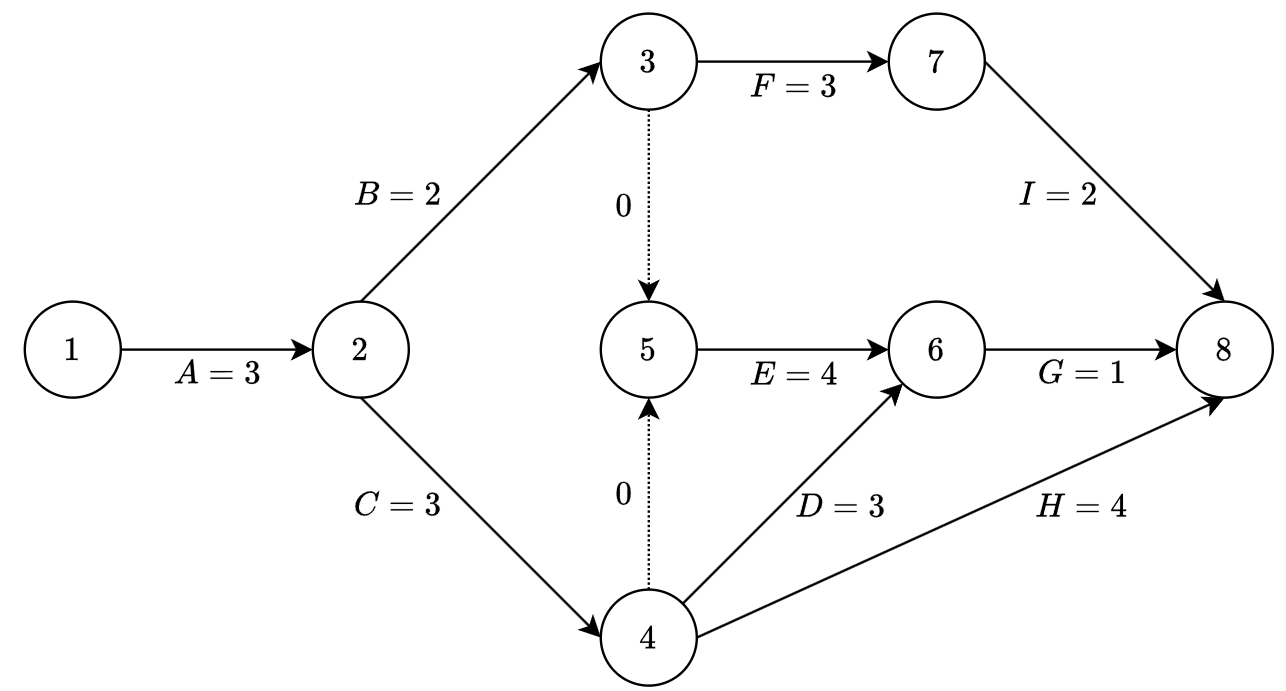
\includegraphics[width=0.5\linewidth]{images/eproject.png}
        \end{figure}
        The first two phases are: 
        \begin{figure}[H]
            \centering
            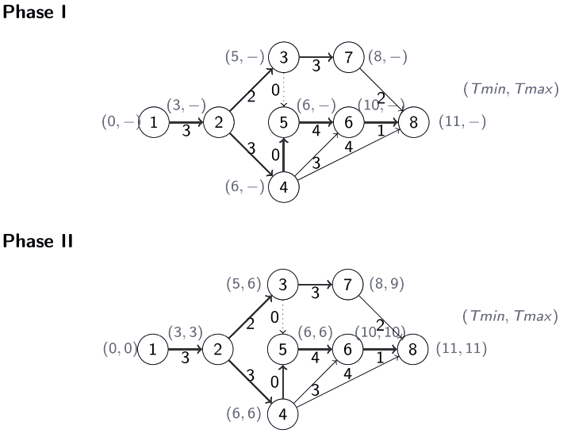
\includegraphics[width=0.75\linewidth]{images/aproject.png}
        \end{figure}
        So, we have that the longest path that is critical is: $(1,2,4,5,6,8)$.
    \end{example}
    This algorithm inputs are: a graph $G = (N,A)$, with $n= \left\lvert N \right\rvert $ and the duration $d_{ij}$ associated to each $(i,j) \in A$. 
    \begin{algorithm}[H]
        \caption{Algorithm for the critical path method}
            \begin{algorithmic}[1]
                \State Sort the nodes of $G$ topologically
                \State $T_{min_1} \leftarrow 0$
                \For {$j=2,\dots,n$}
                    \State $T_{min_j} \leftarrow \max\{T_{min_i}+d_{ij}|(i,j) \in \delta^{-}(j)\}$
                \EndFor
                \State $T_{max_n} \leftarrow T_{min_n}$
                \For {$i=n-1,\dots,1$}
                \State $T_{max_j} \leftarrow \min\{T_{max_j}-d_{ij}|(i,j) \in \delta^{+}(j)\}$
                \EndFor
            \end{algorithmic}
    \end{algorithm}
    The complexity is $O(m)$, where $m = \left\lvert A \right\rvert $. 
    \begin{definition}
        An activity $(i,j)$ with zero slack: 
        \[\sigma_{ij}=T_{max_j}-T_{min_i}-d_{ij}=0\]
        is \emph{critical}. 

        A \emph{critical path} is an $s-t$ path only composed of critical activities (it always exists).
    \end{definition}
    To find the slack of a project it is also possible to use Gantt charts, that were introduced in 1910 by Henry Gantt. It provides a temporal representations of the project. 
    \begin{example}
        The result of the previous example are the following: 
        \begin{table}[H]
            \centering
            \begin{tabular}{cccc}
            \hline
            $(i,j)$ & $d_{ij}$ & $T_{min_i}$ & $T_{max_j}$ \\ \hline
            A       & 3        & 0           & 3           \\
            B       & 2        & 3           & 6           \\
            C       & 3        & 3           & 6           \\
            D       & 3        & 6           & 10          \\
            E       & 4        & 6           & 10          \\
            F       & 3        & 5           & 9           \\
            G       & 1        & 10          & 11          \\
            H       & 4        & 6           & 11          \\
            I       & 2        & 8           & 11          \\ \hline
            \end{tabular}
        \end{table}
        And they can be represented with a Gantt chart as follows: 
        \begin{figure}[H]
            \centering
            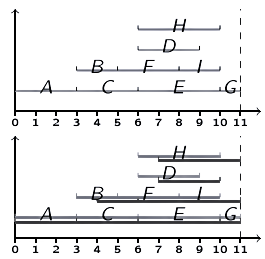
\includegraphics[width=0.4\linewidth]{images/Gantt.png}
        \end{figure}
    \end{example}

    \section{Minimum network flow problem}
    The network flows problems are problem involving the distribution of a given product from a set of sources to a set of users to optimize a given objective function. 
    \begin{definition}
        A network is a directed and connected graph $G = (V,A)$ with a source $s \in V$ and a sink $t \in V$, with $s \neq t$, and a capacity $k_{ij} \geq 0$ for each arc 
        $(i,j) \in A$. 

        A \emph{feasible flow} $x$ from $s$ to $t$ is a vector $x \in \mathbb{R}^m$ with a component $x_{ij}$ for each arc $(i,j) \in A$ satisfying the capacity constraints:
        \[0 \leq x_{ij} \leq k_{ij} \:\:\:\:\:\: \forall (i,j) \in A\]
        and the flow balance constraints at each intermediate node $u \in V (u \neq s,t)$: 
        \[\sum_{(i,u)\in \delta^{-}(u)}x_{iu}=\sum_{(u,j)\in \delta^{+}(u)}x_{uj} \:\:\:\:\:\: \forall u \in N-\{s,t\}\]

        The \emph{value of flow} $x$ is:
        \[\varphi = \sum_{(s,j) \in \delta^{+}(s)} x_{sj}\]

        Given a network and a feasible flow $x$, an arc $(i,j) \in A$ is \emph{saturated} if $x_{ij} = k_{ij}$. 

        Given a network and a feasible flow $x$, an arc $(i,j) \in A$ is \emph{empty} if $x_{ij} = 0$. 
    \end{definition}
    Given a network $G = (V,A)$ with an integer capacity $k_{ij}$ for each arc $(i,j) \in A$, and nodes $s,t \in V$, determine a feasible flow from $s$ to $t$ of maximum value. 

    If there are many sources/sinks with a unique type of product, dummy nodes $s^{*}$ and $t^{*}$ can be added. The linear programming model of the problem is to maximize 
    $max \varphi$ such that: 
    \[\sum_{(u,j)\in \delta^{+}(u)}x_{uj}-\sum_{(i,u)\in \delta^{-}(u)}x_{iu}=
    \begin{cases}
        \varphi \:\:\:\:\:\:\:\:\: u=s    \\
        -\varphi \:\:\:\:\:\: u=t   \\
        0 \:\:\:\:\:\:\:\:\:\: \textnormal{otherwise}
    \end{cases}\]
    where $\varphi$ denotes the value of the feasible flow $x$, $0 \leq x_{ij} \leq k_{ij}$ with $\varphi,x_{ij} \in \mathbb{R}$, and $(i,j) \in A$.
    \begin{definition}
        A \emph{cut separating $s$ from $t$} is $\delta(S)$ of $G$ with $s \in S \subset V$ and $t \in V-S$. There are $2^{n-2}$ cuts separating $s$ from $t$, where 
        $n=\left\lvert V \right\rvert $.

        The \emph{capacity of the cut} $\delta(S)$ induced by $S$ is equal to: 
        \[k(S)=\sum_{(i,j)\in \delta^{+}(S)}k_{ij}\]

        Given a feasible flow $x$ from $s$ to $t$ and a cut $6\delta(S)$ separating $s$ from $t$, the \emph{value of the feasible flow $x$ through the cut $\delta(S)$} is: 
        \[\varphi(S)=\sum_{(i,j)\in \delta^{+}(S)}x_{ij} - \sum_{(i,j)\in \delta^{-}(S)}x_{ij}\]
    \end{definition}
    With this notation the value of the flow $x$ is $\varphi = \varphi(\{s\})$. 
    \begin{example}
        The value of the feasible flow $x$ through the cut $\delta(S)$ in the graph is: 
        \begin{figure}[H]
            \centering
            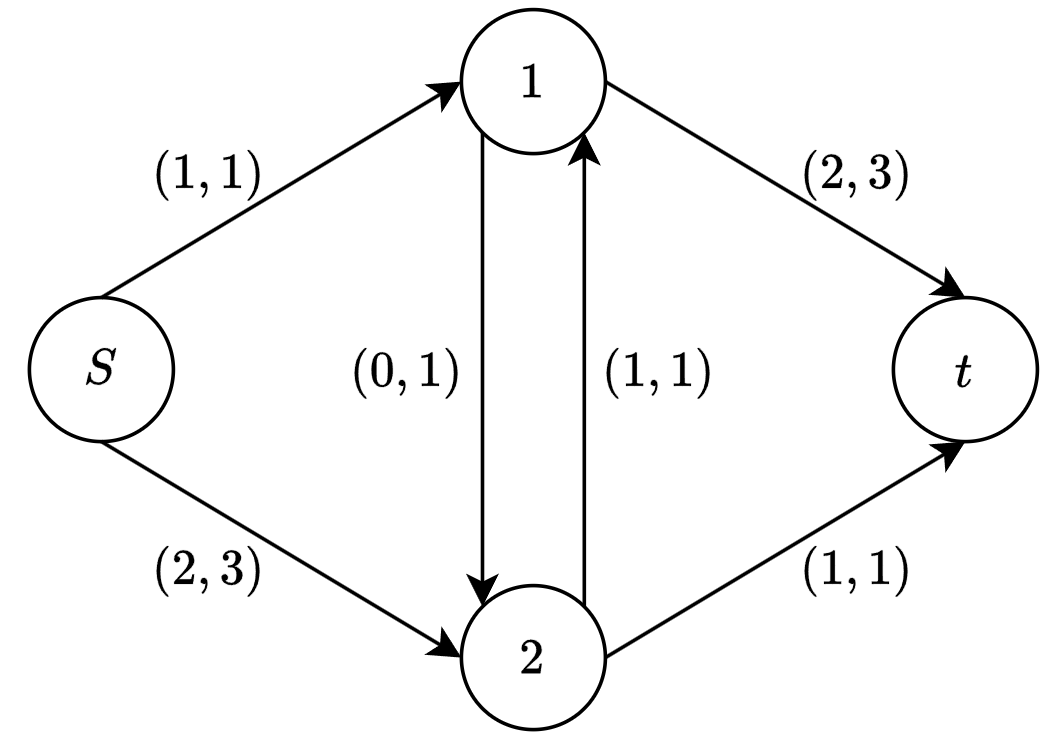
\includegraphics[width=0.4\linewidth]{images/flow.png}
        \end{figure}
        \[\varphi(\{s,1\})=2+0+2-1=3\]
        And the other values are: 
        \[\delta(\{s,1\})=\{(s, 2),(1,2),(1, t)\}\]
        \[k(S)=7\]
    \end{example}
    If $\varphi(S) = k(S)$ for a subset $S \subseteq V$ with $s \in S$ and $t \notin S$, then $x$ is a flow of maximum value and the cut $\delta(S)$ is of minimum capacity. 
    The property $\varphi(S) \leq k(S)$ for any feasible flow $x$ and for any cut $\delta(S)$ separating $s$ from $t$, expresses a weak duality relationship between the two problems:
    \begin{itemize}
        \item Given $G = (V,A)$ with integer capacities on the arcs and $s,t \in V$, determine a feasible flow of maximum value. 
        \item Given $G = (V,A)$ with integer arc capacities and $s,t in V$, determine a cut (separating $s$ from $t$) of minimum capacity. 
    \end{itemize} 

    The idea of the Ford-Fulkerson's algorithm to find the network flows is the following. Start from a feasible flow $x$ and try to iteratively increase its value $\varphi$ by 
    sending, at each iteration, an additional amount of product along an undirected path from $s$ to $t$ with a strictly positive residual capacity. 

    If the arc $(i,j)$ is not saturated we can increase $x_{ij}$. If $(i,j)$ is not empty we can decrease $x_{ij}$ while respecting $0 \leq x_{ij} \leq k_{ij}$. 
    \begin{definition}
        A path $P$ from $s$ to $t$ is an \emph{augmenting path} with respect to the current feasible flow $x$ if $x_{ij} <  k_{ij}$ for any
        forward arc $x_{ij}>0$ for any backward arc. 
    \end{definition}

    Given a feasible flow $x$ for $G=(V,A)$, we construct the residual network $\overline{G}=(V,\overline{A})$ associated to $x$, which 
    accounts for all possible variations of $x$: 
    \begin{itemize}
        \item If $(i,j) \in A$ is not empty $(i,j) \in \overline{A}$ with $\overline{k}_{ij}=x_{ij}>0$.
        \item If $(i,j) \in A$ is not saturated $(i,j) \in \overline{A}$ with $\overline{k}_{ij}=k_{ij}-x_{ij}>0$
    \end{itemize}
    where $\overline{k}_{ij}$ is called the residual capacity. 
    \begin{example}
        The residual capacity of the following graph is computed in this way: 
        \begin{figure}[H]
            \centering
            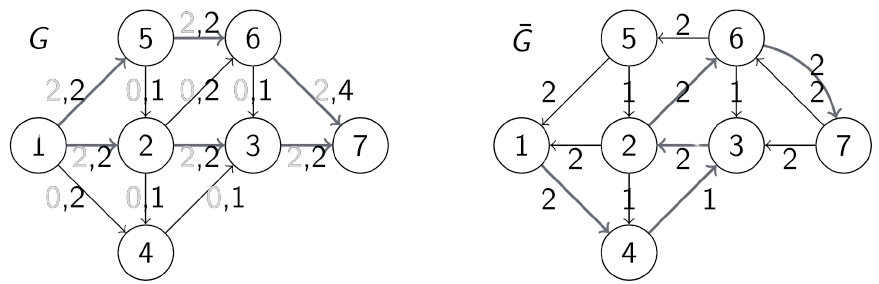
\includegraphics[width=0.75\linewidth]{images/residual1.png}
        \end{figure}
        Then we update the flow, and we calculate again the residual capacity. 
        \begin{figure}[H]
            \centering
            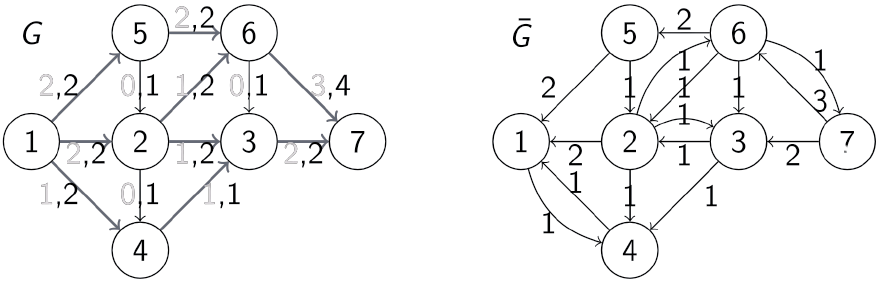
\includegraphics[width=0.75\linewidth]{images/residual2.png}
        \end{figure}
        We do the same process again.
        \begin{figure}[H]
            \centering
            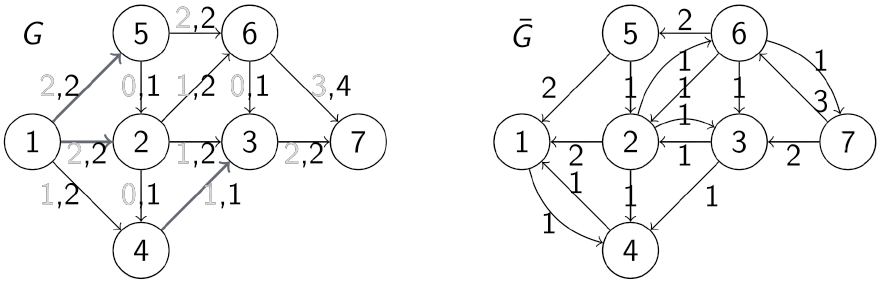
\includegraphics[width=0.75\linewidth]{images/residual3.png}
        \end{figure}
        We cannot find other paths, so we now have obtained that the flow is $\phi=5$.
    \end{example}
    \begin{proposition}
        Ford-Fulkerson's algorithm is exact. 
    \end{proposition}
    \begin{proof}
        A feasible flow $x$ has a maximum value if and only if $t$ is not reachable from $s$ in the residual network associated to $x$. If 
        there is an augmenting path, then $x$ is not optimal for maximum value. If $t$ is not reachable from $s$, then there is a cut of 
        $\overline{G}$ such that $\delta^{+}_{\overline{G}}(S^{*})=\varnothing$. By definition of $\overline{G}$ we have that every 
        $(i,j) \in \delta^{+}_{G}(S^{*})$ is saturated and every $\delta^{-}_{G}(S^{*})$ is empty. Therefore,
        \[\phi(S^{*})=\sum_{(i,j) \in \delta^{+}_{G}(S^{*})}{x_{ij}}-\sum_{(i,j) \in \delta^{-}_{G}(S^{*})}{x_{ij}}=
        \sum_{(i,j) \in \delta^{+}_{G}(S^{*})}{k_{ij}}=k(S^{*})\]
        By weak duality, $\phi(S) < k(S)$, $\forall x$ feasible, $\forall S \subset V$ with $s \in S$, $t \notin S$. Then the flow $x$ has
        maximum value and the cut induced by $S^{*}$ minimum capacity. 
    \end{proof}
    \begin{theorem}[Strong duality]
        The value of a feasible flow of maximum value is equal to the capacity of a cut of minimum capacity.
    \end{theorem}
    The inputs of the algorithm are: a graph $G=(V,A)$ with capacity $k_{ij}>0$ for any $(i,j) \in A$ such that $t \in N$. 
    \begin{algorithm}[H]
        \caption{Ford-Fulkerson's algorithm}
            \begin{algorithmic}[1]
                \State $x \leftarrow 0$
                \State $\phi \leftarrow 0$
                \State $\textnormal{optimum} \leftarrow \textnormal{false}$
                \While {optimum = true}
                    \State Build residual network $\overline{G}$ associated to $x$
                    \State $P \leftarrow$ path from $s$ to $t$ in $\overline{G}$
                    \If {$P$ is not defined}
                        \State optimum $\leftarrow$ true
                    \Else
                        \State $\delta \leftarrow \min\{\overline{k}_{ij}|(i,j) \in P\}$
                        \State $\phi \leftarrow \phi + \delta$
                        \For {$(i,j) \in P$}
                            \If {$(i,j)$ is a forward arc}
                                \State $x_{ij} \leftarrow x_{ij}+\delta$
                            \Else 
                                \State $x_{ij} \leftarrow x_{ij}-\delta$
                            \EndIf
                        \EndFor
                    \EndIf
                \EndWhile
            \end{algorithmic}
    \end{algorithm}
    The overall complexity of this algorithm is $O(m^2k_{max})$. The space complexity of the algorithm is $O(m\log{k_{max}})$. 

    The algorithm can be made polynomial by looking for augmenting path with a minimum number of arcs. 

    \subsection{Minimum cost flow problem}
    Given a network with a unit cost $c_{ij}$ associated to each arc $(i,j)$ and a value $\phi > 0$, determine a feasible flow from $s$ 
    to $t$ of value $\phi$ and of minimum total cost. 

    The idea to solve this problem is to start from a feasible flow $x$ of value $\phi$ and send, an additional amount of product in the
    residual network along cycles of negative cost. 

    \subsection{Assignment problem}
    \begin{definition}
        Given an undirected bipartite graph $G=(V,E)$, a \emph{matching} $M \subseteq E$ is a subset of non-adjacent edges. 
    \end{definition}
    \begin{figure}[H]
        \centering
        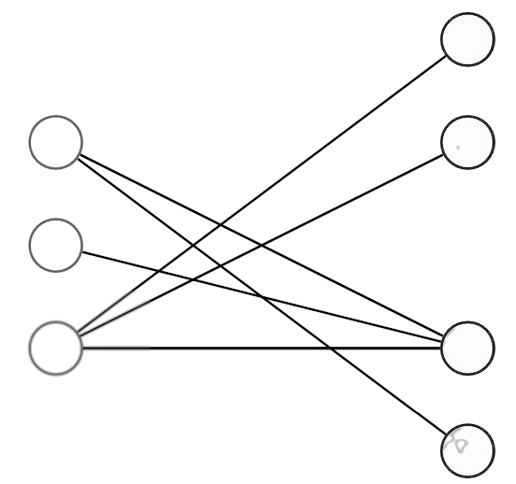
\includegraphics[width=0.25\linewidth]{images/matching.png}
    \end{figure}
    Given a bipartite graph $G=(V,E)$, determine a matching with a maximum number of edges. This problem can be reduced to the problem of
    finding a feasible flow of maximum value from $s$ to $t$ in the following network. 
    \begin{figure}[H]
        \centering
        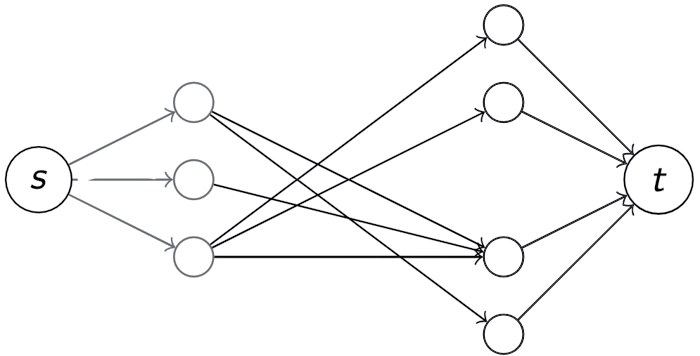
\includegraphics[width=0.25\linewidth]{images/matchingmod.png}
    \end{figure}
    There is a correspondence between the feasible flow of value $\phi$ and the matching containing $\phi$ edges. 
\end{document}